% Options for packages loaded elsewhere
\PassOptionsToPackage{unicode}{hyperref}
\PassOptionsToPackage{hyphens}{url}
%
\documentclass[
  8pt,
  ignorenonframetext,
]{beamer}
\usepackage{pgfpages}
\setbeamertemplate{caption}[numbered]
\setbeamertemplate{caption label separator}{: }
\setbeamercolor{caption name}{fg=normal text.fg}
\beamertemplatenavigationsymbolsempty
% Prevent slide breaks in the middle of a paragraph
\widowpenalties 1 10000
\raggedbottom
\setbeamertemplate{part page}{
  \centering
  \begin{beamercolorbox}[sep=16pt,center]{part title}
    \usebeamerfont{part title}\insertpart\par
  \end{beamercolorbox}
}
\setbeamertemplate{section page}{
  \centering
  \begin{beamercolorbox}[sep=12pt,center]{part title}
    \usebeamerfont{section title}\insertsection\par
  \end{beamercolorbox}
}
\setbeamertemplate{subsection page}{
  \centering
  \begin{beamercolorbox}[sep=8pt,center]{part title}
    \usebeamerfont{subsection title}\insertsubsection\par
  \end{beamercolorbox}
}
\AtBeginPart{
  \frame{\partpage}
}
\AtBeginSection{
  \ifbibliography
  \else
    \frame{\sectionpage}
  \fi
}
\AtBeginSubsection{
  \frame{\subsectionpage}
}
\usepackage{amsmath,amssymb}
\usepackage{lmodern}
\usepackage{iftex}
\ifPDFTeX
  \usepackage[T1]{fontenc}
  \usepackage[utf8]{inputenc}
  \usepackage{textcomp} % provide euro and other symbols
\else % if luatex or xetex
  \usepackage{unicode-math}
  \defaultfontfeatures{Scale=MatchLowercase}
  \defaultfontfeatures[\rmfamily]{Ligatures=TeX,Scale=1}
\fi
% Use upquote if available, for straight quotes in verbatim environments
\IfFileExists{upquote.sty}{\usepackage{upquote}}{}
\IfFileExists{microtype.sty}{% use microtype if available
  \usepackage[]{microtype}
  \UseMicrotypeSet[protrusion]{basicmath} % disable protrusion for tt fonts
}{}
\makeatletter
\@ifundefined{KOMAClassName}{% if non-KOMA class
  \IfFileExists{parskip.sty}{%
    \usepackage{parskip}
  }{% else
    \setlength{\parindent}{0pt}
    \setlength{\parskip}{6pt plus 2pt minus 1pt}}
}{% if KOMA class
  \KOMAoptions{parskip=half}}
\makeatother
\usepackage{xcolor}
\newif\ifbibliography
\usepackage{color}
\usepackage{fancyvrb}
\newcommand{\VerbBar}{|}
\newcommand{\VERB}{\Verb[commandchars=\\\{\}]}
\DefineVerbatimEnvironment{Highlighting}{Verbatim}{commandchars=\\\{\}}
% Add ',fontsize=\small' for more characters per line
\usepackage{framed}
\definecolor{shadecolor}{RGB}{248,248,248}
\newenvironment{Shaded}{\begin{snugshade}}{\end{snugshade}}
\newcommand{\AlertTok}[1]{\textcolor[rgb]{0.94,0.16,0.16}{#1}}
\newcommand{\AnnotationTok}[1]{\textcolor[rgb]{0.56,0.35,0.01}{\textbf{\textit{#1}}}}
\newcommand{\AttributeTok}[1]{\textcolor[rgb]{0.77,0.63,0.00}{#1}}
\newcommand{\BaseNTok}[1]{\textcolor[rgb]{0.00,0.00,0.81}{#1}}
\newcommand{\BuiltInTok}[1]{#1}
\newcommand{\CharTok}[1]{\textcolor[rgb]{0.31,0.60,0.02}{#1}}
\newcommand{\CommentTok}[1]{\textcolor[rgb]{0.56,0.35,0.01}{\textit{#1}}}
\newcommand{\CommentVarTok}[1]{\textcolor[rgb]{0.56,0.35,0.01}{\textbf{\textit{#1}}}}
\newcommand{\ConstantTok}[1]{\textcolor[rgb]{0.00,0.00,0.00}{#1}}
\newcommand{\ControlFlowTok}[1]{\textcolor[rgb]{0.13,0.29,0.53}{\textbf{#1}}}
\newcommand{\DataTypeTok}[1]{\textcolor[rgb]{0.13,0.29,0.53}{#1}}
\newcommand{\DecValTok}[1]{\textcolor[rgb]{0.00,0.00,0.81}{#1}}
\newcommand{\DocumentationTok}[1]{\textcolor[rgb]{0.56,0.35,0.01}{\textbf{\textit{#1}}}}
\newcommand{\ErrorTok}[1]{\textcolor[rgb]{0.64,0.00,0.00}{\textbf{#1}}}
\newcommand{\ExtensionTok}[1]{#1}
\newcommand{\FloatTok}[1]{\textcolor[rgb]{0.00,0.00,0.81}{#1}}
\newcommand{\FunctionTok}[1]{\textcolor[rgb]{0.00,0.00,0.00}{#1}}
\newcommand{\ImportTok}[1]{#1}
\newcommand{\InformationTok}[1]{\textcolor[rgb]{0.56,0.35,0.01}{\textbf{\textit{#1}}}}
\newcommand{\KeywordTok}[1]{\textcolor[rgb]{0.13,0.29,0.53}{\textbf{#1}}}
\newcommand{\NormalTok}[1]{#1}
\newcommand{\OperatorTok}[1]{\textcolor[rgb]{0.81,0.36,0.00}{\textbf{#1}}}
\newcommand{\OtherTok}[1]{\textcolor[rgb]{0.56,0.35,0.01}{#1}}
\newcommand{\PreprocessorTok}[1]{\textcolor[rgb]{0.56,0.35,0.01}{\textit{#1}}}
\newcommand{\RegionMarkerTok}[1]{#1}
\newcommand{\SpecialCharTok}[1]{\textcolor[rgb]{0.00,0.00,0.00}{#1}}
\newcommand{\SpecialStringTok}[1]{\textcolor[rgb]{0.31,0.60,0.02}{#1}}
\newcommand{\StringTok}[1]{\textcolor[rgb]{0.31,0.60,0.02}{#1}}
\newcommand{\VariableTok}[1]{\textcolor[rgb]{0.00,0.00,0.00}{#1}}
\newcommand{\VerbatimStringTok}[1]{\textcolor[rgb]{0.31,0.60,0.02}{#1}}
\newcommand{\WarningTok}[1]{\textcolor[rgb]{0.56,0.35,0.01}{\textbf{\textit{#1}}}}
\setlength{\emergencystretch}{3em} % prevent overfull lines
\providecommand{\tightlist}{%
  \setlength{\itemsep}{0pt}\setlength{\parskip}{0pt}}
\setcounter{secnumdepth}{-\maxdimen} % remove section numbering
\newlength{\cslhangindent}
\setlength{\cslhangindent}{1.5em}
\newlength{\csllabelwidth}
\setlength{\csllabelwidth}{3em}
\newlength{\cslentryspacingunit} % times entry-spacing
\setlength{\cslentryspacingunit}{\parskip}
\newenvironment{CSLReferences}[2] % #1 hanging-ident, #2 entry spacing
 {% don't indent paragraphs
  \setlength{\parindent}{0pt}
  % turn on hanging indent if param 1 is 1
  \ifodd #1
  \let\oldpar\par
  \def\par{\hangindent=\cslhangindent\oldpar}
  \fi
  % set entry spacing
  \setlength{\parskip}{#2\cslentryspacingunit}
 }%
 {}
\usepackage{calc}
\newcommand{\CSLBlock}[1]{#1\hfill\break}
\newcommand{\CSLLeftMargin}[1]{\parbox[t]{\csllabelwidth}{#1}}
\newcommand{\CSLRightInline}[1]{\parbox[t]{\linewidth - \csllabelwidth}{#1}\break}
\newcommand{\CSLIndent}[1]{\hspace{\cslhangindent}#1}
% type setting
% ------------------------------------------------------------------------------
\usepackage[german]{babel}     

% fonts
% ------------------------------------------------------------------------------
\usefonttheme{professionalfonts}

% slide title and horizontal line
% ------------------------------------------------------------------------------
\setbeamertemplate{frametitle}{%
    \vskip-30pt \color{black}\large%
    \begin{minipage}[b][23pt]{120mm}%
    \flushleft\insertframetitle%
    \end{minipage}%
}

\setbeamertemplate{headline}										
{
\vskip10pt\hfill\hspace{3.5mm} 										 
\vskip15pt\color{black}\rule{\textwidth}{0.4pt} 					 
}

% slide number
% ---------------------------------------------------------------
\setbeamertemplate{navigation symbols}{}
\setbeamertemplate{footline}
{
\vskip5pt
\vskip2pt
\makebox[123mm]{\hspace{7.5mm}
\hfill Wahrscheinlichkeitstheorie und Frequentistische Inferenz $\vert$ 
\copyright $ $ 2023 Dirk Ostwald CC BY-SA 4.0 $\vert$ 
Folie \insertframenumber}
\vskip4pt
}

% block color scheme
% ------------------------------------------------------------------------------
% colors
\definecolor{white}{RGB}{255,255,255}
\definecolor{grey}{RGB}{235,235,235}
\definecolor{lightgrey}{RGB}{245,245,245}
\definecolor{LightBlue}{RGB}{220,220,255}
\definecolor{darkblue}{RGB}{51, 51, 153}

% definitions and theorems
\setbeamercolor{block title}{fg = black, bg = grey}
\setbeamercolor{block body}{fg = black, bg = lightgrey}

% general line spacing 
% ------------------------------------------------------------------------------
\linespread{1.3}

% local line spacing
% ------------------------------------------------------------------------------
\usepackage{setspace}

% colors
% -----------------------------------------------------------------------------
\usepackage{color}

% justified text
% ------------------------------------------------------------------------------
\usepackage{ragged2e}
\usepackage{etoolbox}
\apptocmd{\frame}{}{\justifying}{}

% bullet point lists
% -----------------------------------------------------------------------------
\setbeamertemplate{itemize item}[circle]
\setbeamertemplate{itemize subitem}[circle]
\setbeamertemplate{itemize subsubitem}[circle]
\setbeamercolor{itemize item}{fg = black}
\setbeamercolor{itemize subitem}{fg = black}
\setbeamercolor{itemize subsubitem}{fg = black}
\setbeamercolor{enumerate item}{fg = black}
\setbeamercolor{enumerate subitem}{fg = black}
\setbeamercolor{enumerate subsubitem}{fg = black}
\setbeamerfont{itemize/enumerate body}{}
\setbeamerfont{itemize/enumerate subbody}{size = \normalsize}
\setbeamerfont{itemize/enumerate subsubbody}{size = \normalsize}

% color links
% ------------------------------------------------------------------------------
\usepackage{hyperref}
\definecolor{urls}{RGB}{204,0,0}
\hypersetup{colorlinks, citecolor = darkblue, urlcolor = urls}


% additional math commands
% ------------------------------------------------------------------------------
\usepackage{bm}           
\newcommand{\niton}{\not\owns}
\newcommand{\ups}{\upsilon}

% text highlighting
% ------------------------------------------------------------------------------
\usepackage{soul}
\makeatletter
\let\HL\hl
\renewcommand\hl{%
  \let\set@color\beamerorig@set@color
  \let\reset@color\beamerorig@reset@color
  \HL}
\makeatother

% equation highlighting
% -----------------------------------------------------------------------------
\newcommand{\highlight}[2][yellow]{\mathchoice%
  {\colorbox{#1}{$\displaystyle#2$}}%
  {\colorbox{#1}{$\textstyle#2$}}%
  {\colorbox{#1}{$\scriptstyle#2$}}%
  {\colorbox{#1}{$\scriptscriptstyle#2$}}}%

% additional mathematical operators
% ------------------------------------------------------------------------------
\DeclareMathOperator*{\argmax}{arg\,max}
\DeclareMathOperator*{\argmin}{arg\,min}

\ifLuaTeX
  \usepackage{selnolig}  % disable illegal ligatures
\fi
\IfFileExists{bookmark.sty}{\usepackage{bookmark}}{\usepackage{hyperref}}
\IfFileExists{xurl.sty}{\usepackage{xurl}}{} % add URL line breaks if available
\urlstyle{same} % disable monospaced font for URLs
\hypersetup{
  hidelinks,
  pdfcreator={LaTeX via pandoc}}

\author{}
\date{\vspace{-2.5em}}

\begin{document}

\begin{frame}[plain]{}
\protect\hypertarget{section}{}
\center

\begin{center}
\includegraphics[width=0.2\linewidth]{4_Abbildungen/wtfi_4_otto} \end{center}

\vspace{2mm}

\Large

Wahrscheinlichkeitstheorie und Frequentistische Inferenz \vspace{6mm}

\large

BSc Psychologie WiSe 2022/23

\vspace{6mm}
\large

Prof.~Dr.~Dirk Ostwald
\end{frame}

\begin{frame}[plain]{}
\protect\hypertarget{section-1}{}
\vfill
\center
\huge

\textcolor{black}{(4) Zufallsvariablen} \vfill
\end{frame}

\begin{frame}{}
\protect\hypertarget{section-2}{}
\begin{center}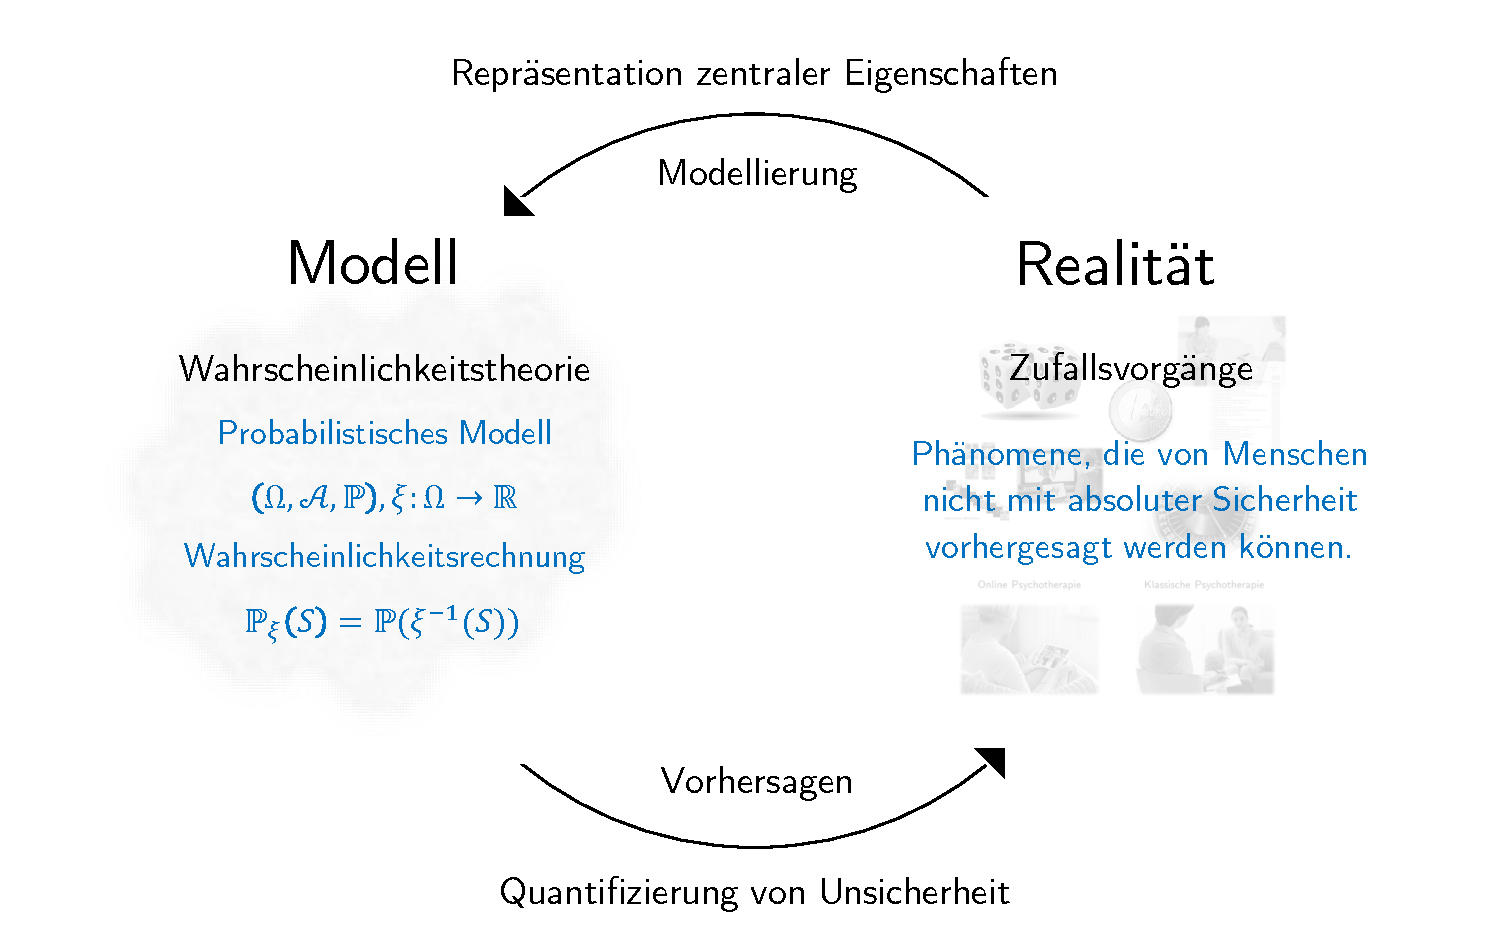
\includegraphics[width=0.95\linewidth]{4_Abbildungen/wtfi_4_wahrscheinlichkeitstheorie_modell} \end{center}
\end{frame}

\begin{frame}{}
\protect\hypertarget{section-3}{}
\begin{center}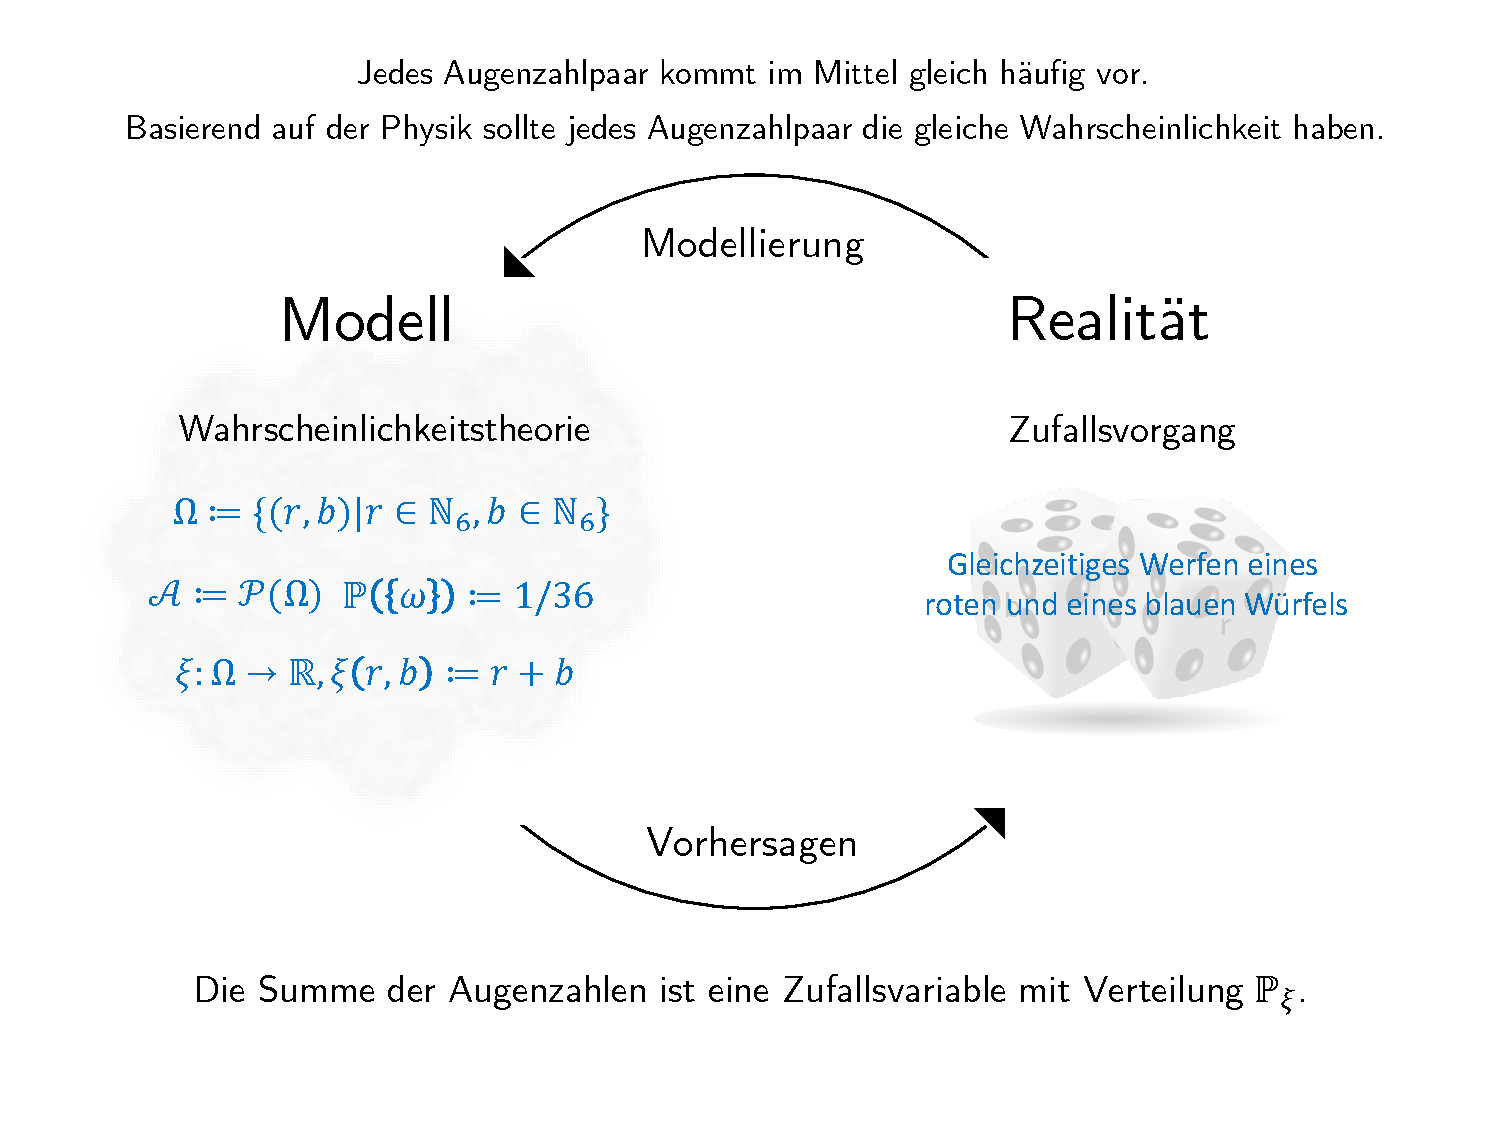
\includegraphics[width=0.9\linewidth]{4_Abbildungen/wtfi_4_wahrscheinlichkeitstheorie_modell_beispiel} \end{center}
\end{frame}

\begin{frame}{}
\protect\hypertarget{section-4}{}
\large
\setstretch{2.7}
\vfill

Konstruktion, Definition, Notation, Intuition

Wahrscheinlichkeitsmassefunktionen

Wahrscheinlichkeitsdichtefunktionen

Kumulative Verteilungsfunktionen

Selbstkontrollfragen \vfill
\end{frame}

\begin{frame}{}
\protect\hypertarget{section-5}{}
\large
\setstretch{2.7}
\vfill

\textbf{Konstruktion, Definition, Notation, Intuition}

Wahrscheinlichkeitsmassefunktionen

Wahrscheinlichkeitsdichtefunktionen

Kumulative Verteilungsfunktionen

Selbstkontrollfragen \vfill
\end{frame}

\begin{frame}{Konstruktion, Definition, Notation, Intuition}
\protect\hypertarget{konstruktion-definition-notation-intuition}{}
Konstruktion von Zufallsvariablen und Verteilungen \small
\setstretch{1.4}

\begin{itemize}
\item Es seien $(\Omega,\mathcal{A},\mathbb{P})$ ein Wahrscheinlichkeitsraum und $\xi : \Omega \to \mathcal{X}$ eine Abbildung.
\item $\xi$ ist das kleine griechische Xi.
\item Es sei $\mathcal{S}$ eine $\sigma$-Algebra auf $\mathcal{X}$.
\item Für jedes $S \in \mathcal{S}$ sei das \textit{Urbild von $S$} definiert als
\begin{equation}
\xi^{-1}(S) := \{\omega \in \Omega|\xi(\omega) \in S\}.
\end{equation}
\item Wenn $\xi^{-1}(S) \in \mathcal{A}$ für alle $S \in \mathcal{S}$ gilt,
dann heißt $\xi$ \textit{messbar}.
\item $\xi : \Omega \to \mathcal{X}$ sei messbar. Allen $S \in \mathcal{S}$
kann die Wahrscheinlichkeit
\begin{equation}
\mathbb{P}_\xi : \mathcal{S} \to [0,1], S \mapsto
\mathbb{P}_\xi(S)
:= \mathbb{P}\left(\xi^{-1}(S)\right)
 = \mathbb{P}\left(\{\omega \in \Omega|\xi(\omega) \in S\}\right)
\end{equation}
zugeordnet werden.
\item $\xi$ heißt nun \textit{Zufallsvariable} und $\mathbb{P}_\xi$ heißt
\textit{Bildmaß} oder \textit{Verteilung von $\xi$}.
\item $(\mathcal{X},\mathcal{S},\mathbb{P}_\xi)$ ist ein Wahrscheinlichkeitsraum.
\item Mit $\mathcal{X} := \mathbb{R}$ und $\mathcal{S} := \mathcal{B}(\mathbb{R})$ rückt der
Wahrscheinlichkeitsraum $(\mathbb{R},\mathcal{B}(\mathbb{R}),\mathbb{P}_\xi)$ ins Zentrum.
\end{itemize}
\end{frame}

\begin{frame}{Konstruktion, Definition, Notation, Intuition}
\protect\hypertarget{konstruktion-definition-notation-intuition-1}{}
\vspace{.2cm}
\center

\begin{center}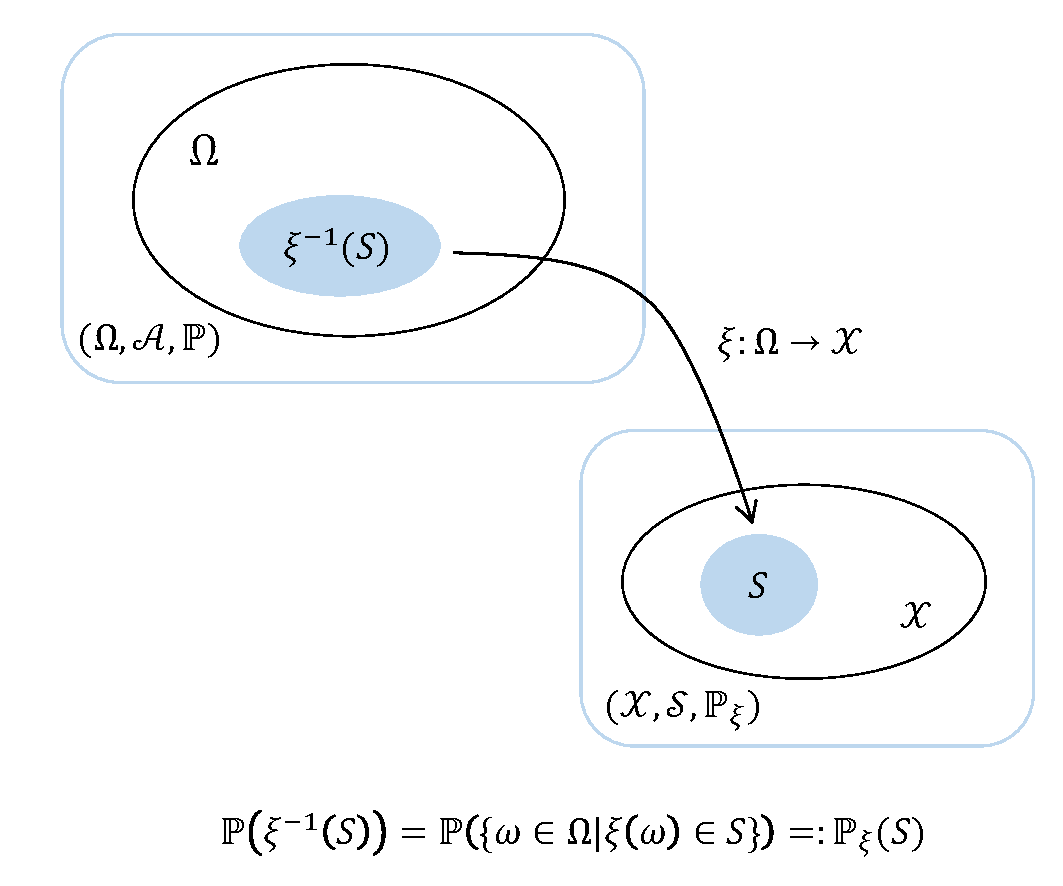
\includegraphics[width=0.7\linewidth]{4_Abbildungen/wtfi_4_zufallsvariable} \end{center}
\end{frame}

\begin{frame}{Konstruktion, Definition, Notation, Intuition}
\protect\hypertarget{konstruktion-definition-notation-intuition-2}{}
\small
\begin{definition}[Zufallsvariable]
\justifying
Es sei $(\Omega, \mathcal{A}, \mathbb{P})$ ein Wahrscheinlichkeitsraum und
$(\mathcal{X},\mathcal{S})$ ein \textit{Messraum}. Dann ist eine \textit{Zufallsvariable (ZV)}
definiert als eine Abbildung $\xi:\Omega \to \mathcal{X}$ mit der \textit{Messbarkeitseigenschaft}
\begin{equation}
\{\omega \in \Omega|\xi(\omega) \in S \} \in \mathcal{A} \mbox{ für alle } S \in \mathcal{S}.
\end{equation}
\end{definition}

Bemerkungen

\begin{itemize}
\justifying
\item ZVen sind weder ``zufällig'' noch ``Variablen''.
\item Intuitiv wird $\omega \in \Omega$ ``zufällig'' anhand von $\mathbb{P}$
gezogen und $\xi(\omega)$ realisiert.
\item Wir nennen $\mathcal{X}$ den \textit{Ergebnisraum der ZV $\xi$}.
\item Die Verteilungen (Bildmaße) von ZVen sind in der Statistik zentral.
\item Der Begriff der Verteilung wird oft auch für W-Maße und Dichten verwendet.
\end{itemize}
\end{frame}

\begin{frame}{Konstruktion, Definition, Notation, Intuition}
\protect\hypertarget{konstruktion-definition-notation-intuition-3}{}
Beispiel (Summe eines roten und eines blauen Würfels) \vspace{1mm}

\small
\begin{itemize}
\justifying
\item Für das Werfen zweier Würfel ist ein sinnvolles Wahrscheinlichkeitsraum-Modell
\begin{itemize}
\small
\item $\Omega := \{(r,b)| r  \in \mathbb{N}_6, b \in \mathbb{N}_6\}$
\item $\mathcal{A} := \mathcal{P}(\Omega)$.
\item $\mathbb{P} : \mathcal{A} \to [0,1]$ mit $\mathbb{P}(\{(r,b)\}) = 1/36$ für alle $(r,b) \in \Omega$.

\end{itemize}

\item Die Augenzahl-Summenbildung wird dann sinnvoller Weise durch die Zufallsvariable
\begin{equation}
\xi : \Omega \to \mathcal{X}, (r,b) \mapsto \xi((r,b)) := r + b.
\end{equation}
beschrieben, wobei $\mathcal{X} := \{2,3,...,12\}$.

\item $\mathcal{S} := \mathcal{P}(\mathcal{X})$ ist eine sinnvolle $\sigma$-Algebra auf $\mathcal{X}$.

\item Mithilfe der $\sigma$-Addivität von $\mathbb{P}$ können wir die Verteilung
$\mathbb{P}_\xi$ von $\xi$ für alle Elementarereignisse $\{x\} \in \mathcal{S}$ berechnen,
wie auf der nächsten Folie gezeigt.
\item Wir haben damit ein weiteres Wahrscheinlichkeitsraum-Modell
$(\mathcal{X}, \mathcal{S}, \mathbb{P}_\xi)$ konstruiert.
\end{itemize}
\end{frame}

\begin{frame}{Konstruktion, Definition, Notation, Intuition}
\protect\hypertarget{konstruktion-definition-notation-intuition-4}{}
Beispiel (Summe zweier Würfel) \vspace{1mm} \small

Bestimmung der Verteilung \(\mathbb{P}_\xi\) von \(\xi\) \vspace{2mm}

\footnotesize
\renewcommand{\arraystretch}{1.5}
\begin{tabular}{llll}

  $\mathbb{P}_\xi(\{2\})$
& $ = \mathbb{P}\left(\xi^{-1}(\{2\})\right)$
& $ = \mathbb{P}\left(\{(1,1)\}\right)$
& $ = \frac{1}{36}$
\\
  $\mathbb{P}_\xi(\{3\})$
& $ = \mathbb{P}\left(\xi^{-1}(\{3\})\right)$
& $ = \mathbb{P}\left(\{(1,2),(2,1)\}\right)$
& $ = \frac{2}{36}$
\\
  $\mathbb{P}_\xi(\{4\})$
& $ = \mathbb{P}\left(\xi^{-1}(\{4\})\right)$
& $ = \mathbb{P}\left(\{(1,3),(3,1),(2,2)\}\right)$
& $ = \frac{3}{36}$
\\
  $\mathbb{P}_\xi(\{5\})$
& $ = \mathbb{P}\left(\xi^{-1}(\{5\})\right)$
& $ = \mathbb{P}\left(\{(1,4),(4,1),(2,3),(3,2)\}\right)$
& $ = \frac{4}{36}$
\\
  $\mathbb{P}_\xi(\{6\})$
& $ = \mathbb{P}\left(\xi^{-1}(\{6\})\right)$
& $ = \mathbb{P}\left(\{(1,5),(5,1),(2,4),(4,2),(3,3)\}\right)$
& $ = \frac{5}{36}$
\\
  $\mathbb{P}_\xi(\{7\})$
& $ = \mathbb{P}\left(\xi^{-1}(\{7\})\right)$
& $ = \mathbb{P}\left(\{(1,6),(6,1),(2,5),(5,2),(3,4),(4,3)\}\right)$
& $ = \frac{6}{36}$
\\
  $\mathbb{P}_\xi(\{8\})$
& $ = \mathbb{P}\left(\xi^{-1}(\{8\})\right)$
& $ = \mathbb{P}\left(\{(2,6),(6,2),(3,5),(5,3),(4,4)\}\right)$
& $ = \frac{5}{36}$
\\
  $\mathbb{P}_\xi(\{9\})$
& $ = \mathbb{P}\left(\xi^{-1}(\{9\})\right)$
& $ = \mathbb{P}\left(\{(3,6),(6,3),(4,5),(5,4)\}\right)$
& $ = \frac{4}{36}$
\\
  $\mathbb{P}_\xi(\{10\})$
& $ = \mathbb{P}\left(\xi^{-1}(\{10\})\right)$
& $ = \mathbb{P}\left(\{(4,6),(6,4),(5,5)\}\right)$
& $ = \frac{3}{36}$
\\
  $\mathbb{P}_\xi(\{11\})$
& $ = \mathbb{P}\left(\xi^{-1}(\{11\})\right)$
& $ = \mathbb{P}\left(\{(5,6),(6,5)\}\right)$
& $ = \frac{2}{36}$
\\
  $\mathbb{P}_\xi(\{12\})$
& $ = \mathbb{P}\left(\xi^{-1}(\{12\})\right)$
& $ = \mathbb{P}\left(\{(6,6)\}\right)$
& $ = \frac{1}{36}$
\end{tabular}
\end{frame}

\begin{frame}{Konstruktion, Definition, Notation, Intuition}
\protect\hypertarget{konstruktion-definition-notation-intuition-5}{}
\small
\begin{definition}[Notation für Zufallsvariablen]
\justifying
Es seien $(\Omega,\mathcal{A},\mathbb{P})$ und $(\mathcal{X},\mathcal{S},\mathbb{P}_\xi)$
W-Räume und $\xi : \Omega \to \mathcal{X}$ sei eine ZV. Dann gelten folgende Konventionen:
\begin{align*}
\begin{split}
\{\xi \in S\} & := \{\omega \in \Omega|\xi(\omega) \in S\}, S \subset \mathcal{X},  \\
\{\xi  =  x\} & := \{\omega \in \Omega|\xi(\omega)  =  x\}, x \in     \mathcal{X},  \\
\{\xi \le x\} & := \{\omega \in \Omega|\xi(\omega) \le x\}, x \in     \mathcal{X},  \\
\{\xi  <  x\} & := \{\omega \in \Omega|\xi(\omega)  <  x\}, x \in     \mathcal{X}.  \\
\end{split}
\end{align*}
Aus diesen Konventionen folgen exemplarisch die folgenden Konventionen für Verteilungen:
\begin{align*}
\begin{split}
\mathbb{P}_\xi\left(\xi \in S\right)
& = \mathbb{P}\left(\{\xi \in S\} \right)
  = \mathbb{P}\left( \{\omega \in \Omega|\xi(\omega) \in S\} \right), S \subset\mathcal{X}  \\
\mathbb{P}_\xi\left(\xi \le x \right)
& = \mathbb{P}\left(\{\xi \le x\} \right)
  = \mathbb{P}\left( \{\omega \in \Omega|\xi(\omega) \le x\} \right), x \in \mathcal{X}.  \\
\end{split}
\end{align*}
Oft wird zudem auf das ZV Subskript bei Verteilungssymbolen verzichtet, z.B.
\begin{align*}
\begin{split}
\mathbb{P}\left(\xi\in S\right) = \mathbb{P}_\xi\left(\xi \in S\right), S \subset \mathcal{X} , \\
\mathbb{P}\left(\xi\le x\right) = \mathbb{P}_\xi\left(\xi \le S\right), x \in \mathcal{X}.          \\
\end{split}
\end{align*}
\end{definition}
\end{frame}

\begin{frame}[fragile]{Konstruktion, Definition, Notation, Intuition}
\protect\hypertarget{konstruktion-definition-notation-intuition-6}{}
\small
\vspace{2mm}
\begin{definition}[Realisierung einer Zufallsvariable]
\justifying
$(\Omega, \mathcal{A}, \mathbb{P})$ sei ein Wahrscheinlichkeitsraum
$(\mathcal{X},\mathcal{S})$ sei ein Messraum und $\xi : \Omega \to \mathcal{X}$
sei eine Zufallsvariable. Dann heißt $\xi(\omega) \in \mathcal{X}$ auch
\textit{Realisierung der Zufallvariable}.
\end{definition}
\footnotesize

\begin{itemize}
\tightlist
\item
  In der Datenanalyse werden Daten typischerweise als Realisierungen von
  Zufallsvariablen modelliert.
\item
  Da die Auswahl eines \(\omega \in \Omega\) in einem Zufallsvorgang
  zufällig ist, erscheint \(\xi(\omega)\) zufällig.
\end{itemize}

\small

\textcolor{darkblue}{Simulation von Zufallsvariablenrealisierungen (Summe zweier Würfel)}
\vspace{1mm} \footnotesize \setstretch{0.9}

\begin{Shaded}
\begin{Highlighting}[]
\CommentTok{\# Wahrscheinlichkeitsraummodell}
\NormalTok{Omega    }\OtherTok{=} \FunctionTok{list}\NormalTok{()                                 }\CommentTok{\# Ergebnisrauminitialisierung}
\NormalTok{idx      }\OtherTok{=} \DecValTok{1}                                      \CommentTok{\# Ergebnisindexinitialisierung}
\ControlFlowTok{for}\NormalTok{(r }\ControlFlowTok{in} \DecValTok{1}\SpecialCharTok{:}\DecValTok{6}\NormalTok{)\{                                    }\CommentTok{\# Ergebnisse roter  Würfel}
    \ControlFlowTok{for}\NormalTok{(b }\ControlFlowTok{in} \DecValTok{1}\SpecialCharTok{:}\DecValTok{6}\NormalTok{)\{                                }\CommentTok{\# Ergebnisse blauer Würfel}
\NormalTok{        Omega[[idx]] }\OtherTok{=} \FunctionTok{c}\NormalTok{(r,b)                     }\CommentTok{\# \textbackslash{}omega \textbackslash{}in \textbackslash{}Omega}
\NormalTok{        idx          }\OtherTok{=}\NormalTok{ idx }\SpecialCharTok{+} \DecValTok{1}\NormalTok{ \}\}                 }\CommentTok{\# Ergebnisindexupdate}
\NormalTok{K        }\OtherTok{=} \FunctionTok{length}\NormalTok{(Omega)                          }\CommentTok{\# Kardinalität von \textbackslash{}Omega}
\NormalTok{pi       }\OtherTok{=} \FunctionTok{rep}\NormalTok{(}\DecValTok{1}\SpecialCharTok{/}\NormalTok{K,}\DecValTok{1}\NormalTok{,K)                           }\CommentTok{\# Wahrscheinlichkeitsfunktion \textbackslash{}pi}

\CommentTok{\# Zufallsvorgang}
\NormalTok{omega    }\OtherTok{=}\NormalTok{ Omega[[}\FunctionTok{which}\NormalTok{(}\FunctionTok{rmultinom}\NormalTok{(}\DecValTok{1}\NormalTok{,}\DecValTok{1}\NormalTok{,pi) }\SpecialCharTok{==} \DecValTok{1}\NormalTok{)]] }\CommentTok{\# Auswahl von \textbackslash{}omega anhand \textbackslash{}mathbb\{P\}(\{\textbackslash{}omega\})}

\CommentTok{\# Auswertung der Zufallsvariable}
\NormalTok{xi\_omega }\OtherTok{=} \FunctionTok{sum}\NormalTok{(omega)                             }\CommentTok{\# \textbackslash{}xi(\textbackslash{}omega)}
\end{Highlighting}
\end{Shaded}

\setstretch{0.9}

\begin{verbatim}
> omega     :  4 2 
> xi(omega) :  6
\end{verbatim}
\end{frame}

\begin{frame}{Konstruktion, Definition, Notation, Intuition}
\protect\hypertarget{konstruktion-definition-notation-intuition-7}{}
\vspace{1mm}

\textcolor{darkblue}{Zufallsvariablen als Modelle von Messvorgängen}
\vspace{-1mm} \footnotesize \setstretch{0.9}

\begin{center}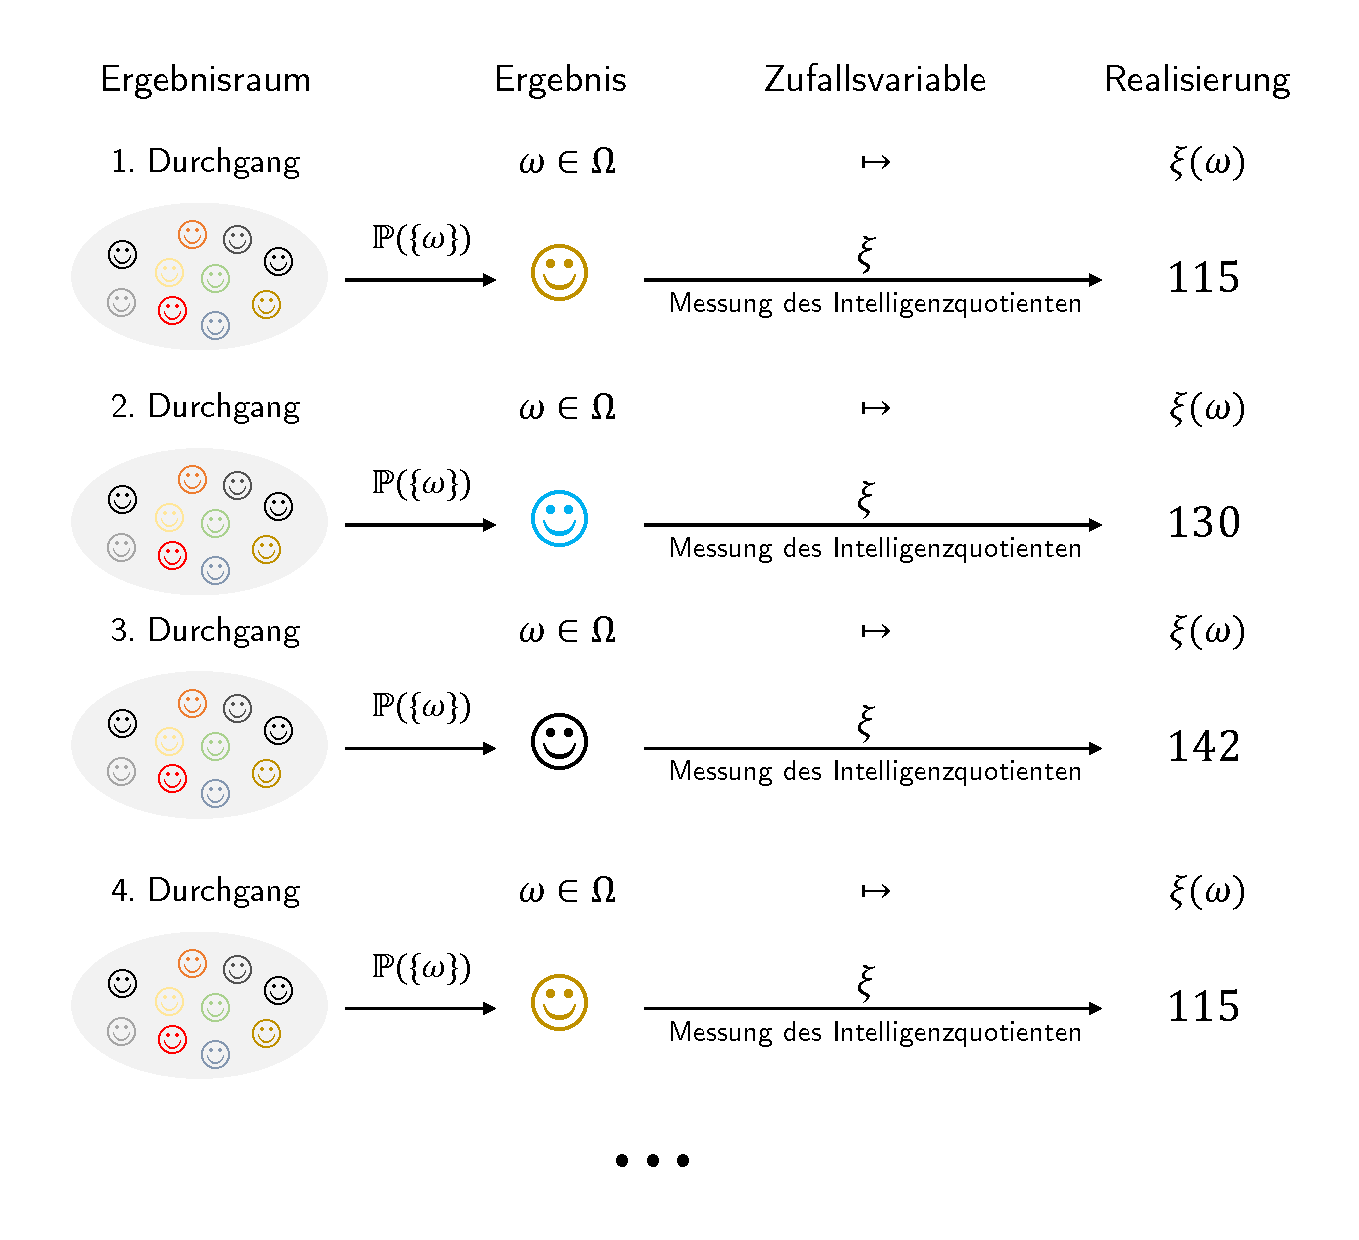
\includegraphics[width=0.7\linewidth]{4_Abbildungen/wtfi_4_zufallsvariable_messen} \end{center}
\end{frame}

\begin{frame}{Konstruktion, Definition, Notation, Intuition}
\protect\hypertarget{konstruktion-definition-notation-intuition-8}{}
\footnotesize
\begin{theorem}[Arithmetik reeller Zufallsvariablen]
\justifying
\normalfont
$(\Omega, \mathcal{A}, \mathbb{P})$ sei ein Wahrscheinlichkeitsraum, 
$(\mathbb{R}, \mathcal{B}(\mathbb{R}))$ sei der reelle Messraum, 
$\xi : \Omega \to \mathbb{R}$, $\ups : \Omega \to  \mathbb{R}$ seien reellwertige 
Zufallsvariablen und $c \in \mathbb{R}$ sei eine Konstante. Weiterhin seien
\begin{align}
\begin{split}
\xi + c    & : \Omega \to \mathbb{R}, \omega \mapsto (\xi + c)(\omega)\,           := \xi(\omega) + c              \mbox{ für } c \in \mathbb{R}   \\
c\xi       & : \Omega \to \mathbb{R}, \omega \mapsto (c\xi)(\omega) \quad\,\,\,    := c\xi(\omega)                 \mbox{ für } c \in \mathbb{R}   \\
\xi + \ups & : \Omega \to \mathbb{R}, \omega \mapsto (\xi + \ups)(\omega)          := \xi(\omega) + \ups(\omega)                                   \\
\xi\ups    & : \Omega \to \mathbb{R}, \omega \mapsto (\xi\ups)(\omega)\quad\,\,\,  := \xi(\omega)\ups(\omega)                                      \\
\end{split}
\end{align}
die Addition einer Konstante zu einer reellwertigen Zufallsvariable, die Multiplikation einer
reellwertigen  Zufallsvariable mit einer Konstante, die Addition zweier reellwertiger Zufallsvariablen und die
Multiplikation zweier reellwertigen Zufallsvariablen, respektive. Dann sind auch $\xi + c$, $c\xi$,
$\xi + \ups$ und $\xi\ups$ reellwertige Zufallsvariablen.
\end{theorem}

Bemerkungen

\begin{itemize}
\tightlist
\item
  Intuitiv ergibt die Addition einer zufälligen Größe zu einer
  konstanten Größe eine zufällige Größe.
\item
  Intuitiv ergibt die Multiplikation einer zufälligen Größe mit einer
  Konstante eine zufällige Größe.
\item
  Intuitiv ergibt die Addition zweier zufälliger Größen wiederum eine
  zufällige Größe.
\item
  Intuitiv ergibt die Multiplikation zweier zufälliger Größen wiederum
  eine zufällige Größe.
\item
  Für einen Beweis, siehe Hesse (2009), Seite 33-34.
\end{itemize}
\end{frame}

\begin{frame}{}
\protect\hypertarget{section-6}{}
\large
\setstretch{2.7}
\vfill

Konstruktion, Definition, Notation, Intuition

\textbf{Wahrscheinlichkeitsmassefunktionen}

Wahrscheinlichkeitsdichtefunktionen

Kumulative Verteilungsfunktionen

Selbstkontrollfragen \vfill
\end{frame}

\begin{frame}{Wahrscheinlichkeitsmassefunktionen}
\protect\hypertarget{wahrscheinlichkeitsmassefunktionen}{}
\small
\begin{definition}[Diskrete ZV, Wahrscheinlichkeitsmassefunktion]
\justifying
Eine Zufallsvariable $\xi$ heißt \textit{diskret}, wenn ihr Ergebnisraum $\mathcal{X}$
endlich oder abzählbar ist und eine Funktion der Form
\begin{equation}
p: \mathcal{X} \to \mathbb{R}_{\ge 0}, x \mapsto p(x)
\end{equation}
existiert, für die gilt
\begin{itemize}
\item[(1)] $\sum_{x \in \mathcal{X}} p(x) = 1$ und
\item[(2)] $\mathbb{P}_\xi(\xi = x) = p(x)$ für alle $x \in \mathcal{X}$.
\end{itemize}
Eine entsprechende Funktion $p$ heißt \textit{Wahrscheinlichkeitsmassefunktion (WMF)} von $\xi$.
\end{definition}

\footnotesize

Bemerkungen

\begin{itemize}
\tightlist
\item
  Eine Menge heißt abzählbar, wenn sie bijektiv auf \(\mathbb{N}\)
  abgebildet werden kann.
\item
  WMFen heißen im Deutschen auch \textit{W-Funktionen} oder
  \textit{Zähldichten}.
\item
  WMFen heißen auf Englisch \textit{probability mass functions (PMFs)}.
\item
  Die Eigenschaft \(\sum_{x \in \mathcal{X}} p(x) = 1\) nennt man auch
  \textit{Normiertheit} von \(p\).
\item
  Zur Parallelität mit PMFs und WDFs bevorzugen wird den Begriff WMF.
\end{itemize}
\end{frame}

\begin{frame}{Wahrscheinlichkeitsmassefunktionen}
\protect\hypertarget{wahrscheinlichkeitsmassefunktionen-1}{}
\small
\begin{definition}[Bernoulli-Zufallsvariable]
\justifying
Es sei $\xi$ eine Zufallsvariable mit Ergebnisraum $\mathcal{X} = \{0,1\}$ und WMF
\begin{equation}
p : \mathcal{X} \to [0,1], x\mapsto p(x) := \mu^{x}(1 - \mu)^{1-x} \mbox{ mit } \mu \in [0,1].
\end{equation}

Dann sagen wir, dass $\xi$ einer \textit{Bernoulli-Verteilung mit Parameter
$\mu \in [0,1]$} unterliegt und nennen $\xi$ eine \textit{Bernoulli-Zufallsvariable}.
Wir kürzen dies mit $\xi \sim \mbox{Bern}(\mu)$ ab. Die WMF einer
Bernoulli-Zufallsvariable bezeichnen wir mit
\begin{equation}
\mbox{Bern}(x;\mu) := \mu^x (1 - \mu)^{1 - x}.
\end{equation}
\end{definition}

Bemerkungen

\begin{itemize}
\justifying
\item Eine Bernoulli-Zufallsvariable kann als Modell eines Münzwurfs dienen.
\item $\mu$ ist die Wahrscheinlichkeit dafür, dass $\xi$ den Wert 1 annimmt,
\begin{equation}
\mathbb{P}(\xi = 1) = \mu^1 (1 -\mu)^{1-1} = \mu.
\end{equation}
\end{itemize}
\end{frame}

\begin{frame}{Wahrscheinlichkeitsmassefunktionen}
\protect\hypertarget{wahrscheinlichkeitsmassefunktionen-2}{}
Bernoulli-Zufallsvariable \vspace{1cm}

\begin{center}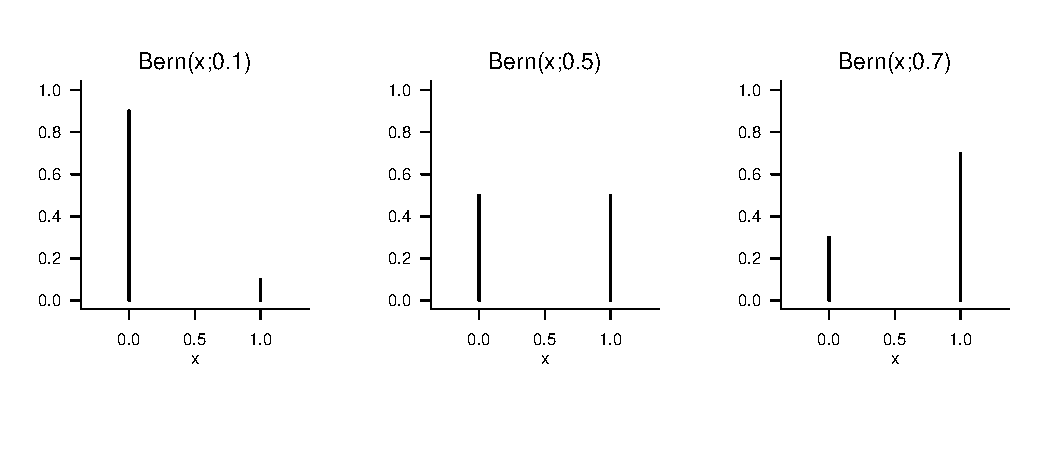
\includegraphics[width=1\linewidth]{4_Abbildungen/wtfi_4_bernoulliverteilung_wmf} \end{center}
\end{frame}

\begin{frame}{Wahrscheinlichkeitsmassefunktionen}
\protect\hypertarget{wahrscheinlichkeitsmassefunktionen-3}{}
\small
\begin{definition}[Binomial-Zufallsvariable]
\vspace{2pt}
\justifying

Es sei $\xi$ eine Zufallsvariable mit Ergebnisraum $\mathcal{X} := \mathbb{N}_n^0$
und WMF
\begin{equation}
p : \mathcal{X} \to [0,1],
x\mapsto p(x) :=
\begin{pmatrix}
n \\ x
\end{pmatrix}
\mu^{x}(1 - \mu)^{n-x} \mbox{ für } \mu \in [0,1].
\end{equation}
Dann sagen wir, dass $\xi$ einer \textit{Binomialverteilung mit Parametern $\mu \in [0,1]$
und $n \in \mathbb{N}$} unterliegt und nennen $\xi$ eine Binomial-Zufallsvariable.
Wir kürzen dies mit $\xi \sim \mbox{Bin}(\mu,n)$ ab. Die WMF einer
Binomial-Zufallsvariable bezeichnen wir mit
\begin{equation}
\mbox{Bin}(x;\mu,n) :=
\begin{pmatrix}
n \\ x
\end{pmatrix}
\mu^{x}(1 - \mu)^{n-x}.
\end{equation}
\end{definition}

Bemerkung

\begin{itemize}
\item Es gilt $\mbox{Bin}(x;\mu,1) = \mbox{Bern}(x;\mu)$.
\end{itemize}
\end{frame}

\begin{frame}{Wahrscheinlichkeitsmassefunktionen}
\protect\hypertarget{wahrscheinlichkeitsmassefunktionen-4}{}
Binomial-Zufallsvariable \vspace{1cm}

\begin{center}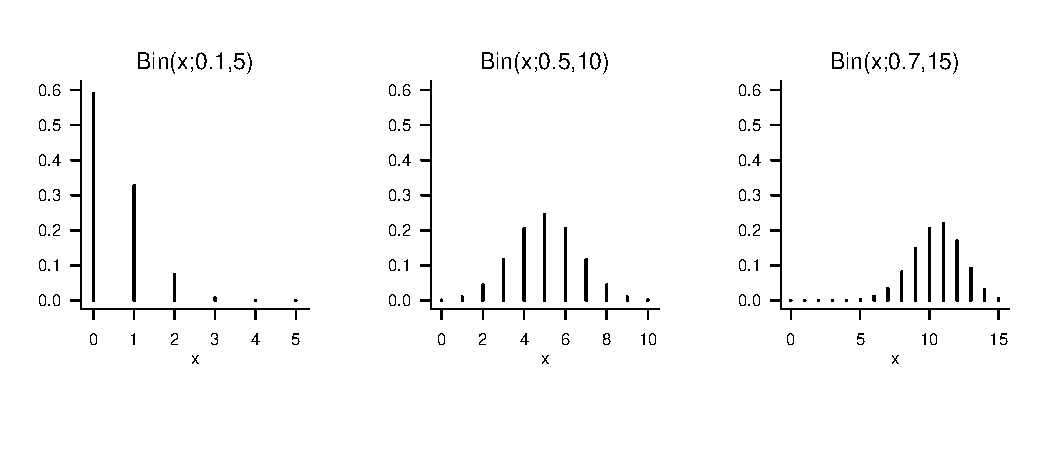
\includegraphics[width=1\linewidth]{4_Abbildungen/wtfi_4_binomialverteilung_wmf} \end{center}
\end{frame}

\begin{frame}{Wahrscheinlichkeitsmassefunktionen}
\protect\hypertarget{wahrscheinlichkeitsmassefunktionen-5}{}
\small
\begin{definition}[Diskret-gleichverteilte Zufallsvariable]
\justifying
Es sei $\xi$ eine diskrete Zufallsvariable mit endlichem Ergebnisraum $\mathcal{X}$ und WMF
\begin{equation}
p : \mathcal{X} \to \mathbb{R}_{\ge 0}, x\mapsto p(x) := \frac{1}{|\mathcal{X}|}.
\end{equation}

Dann sagen wir, dass $\xi$ einer \textit{diskreten Gleichverteilung} unterliegt
und nennen $\xi$ eine \textit{diskret-gleichverteilte Zufallsvariable}. Wir kürzen
dies mit $\xi \sim U(|\mathcal{X}|)$ ab. Die WMF einer diskret-gleichverteilten
Zufallsvariable bezeichnen wir mit
\begin{equation}
U(x;|\mathcal{X}|) := \frac{1}{|\mathcal{X}|}.
\end{equation}
\end{definition}

Bemerkungen

\begin{itemize}
\item $\mbox{Bern}(x;0.5) = U(x;|\mathcal{X}|)$ für $\mathcal{X} = \{0,1\}$.
\end{itemize}
\end{frame}

\begin{frame}{Wahrscheinlichkeitsmassefunktionen}
\protect\hypertarget{wahrscheinlichkeitsmassefunktionen-6}{}
Diskret-gleichverteilte Zufallsvariable \vspace{1cm}

\begin{center}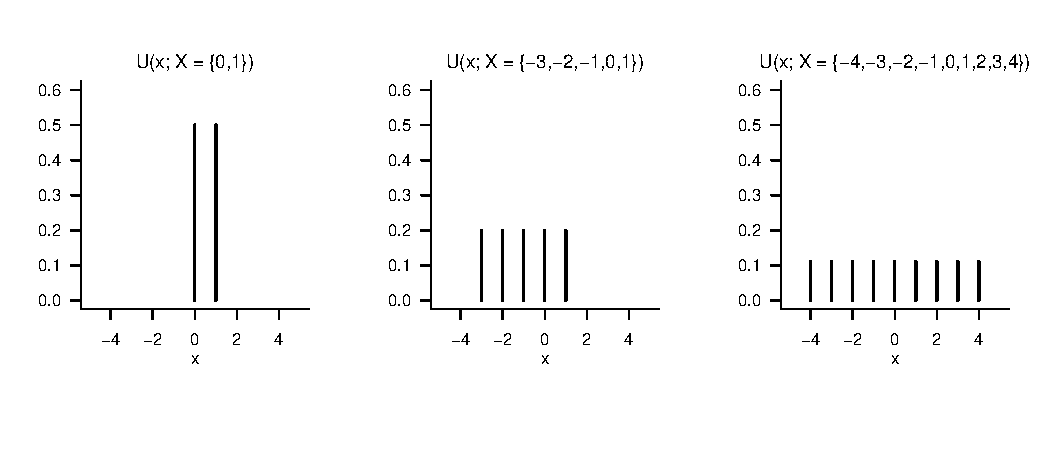
\includegraphics[width=1\linewidth]{4_Abbildungen/wtfi_4_gleichverteilung_wmf} \end{center}
\end{frame}

\begin{frame}{}
\protect\hypertarget{section-7}{}
\large
\setstretch{2.7}
\vfill

Konstruktion, Definition, Notation, Intuition

Wahrscheinlichkeitsmassefunktionen

\textbf{Wahrscheinlichkeitsdichtefunktionen}

Kumulative Verteilungsfunktionen

Selbstkontrollfragen \vfill
\end{frame}

\begin{frame}{Wahrscheinlichkeitsdichtefunktionen}
\protect\hypertarget{wahrscheinlichkeitsdichtefunktionen}{}
\small
\begin{definition}[Kontinuierliche ZV, Wahrscheinlichkeitsdichtefunktion]
Eine Zufallsvariable $\xi$ heißt \textit{kontinuierlich}, wenn eine Funktion der Form
\begin{equation}
p: \mathbb{R} \to \mathbb{R}_{\ge 0}, x \mapsto p(x)
\end{equation}
existiert, für die gilt
\begin{itemize}
\item[(1)] $\int_{-\infty}^{\infty}p(x)dx = 1$,
\item[(2)] $\mathbb{P}_\xi(\xi \in [a,b]) = \int_a^b p(x)\,dx$ für alle $a,b\in\mathbb{R}$ mit $a \le b$.
\end{itemize}
Eine entsprechende Funktion $p$ heißt \textit{Wahrscheinlichkeitsdichtefunktion (WDF)} von $\xi$.
\end{definition}

Bemerkungen

\begin{itemize}
\justifying
\item WDFen können Werte größer als $1$ annehmen.
\item Es gilt $\mathbb{P}_\xi(\xi = a) = \int_a^a p(x) \,dx = 0$.
\item Wahrscheinlichkeiten werden aus WDFen durch Integration berechnet.
\item (Wahrscheinlichkeits)Masse = (Wahrscheinlichkeits)Dichte $\times$ (Mengen)Volumen.
\end{itemize}
\end{frame}

\begin{frame}{Wahrscheinlichkeitsdichtefunktionen}
\protect\hypertarget{wahrscheinlichkeitsdichtefunktionen-1}{}
\small
\begin{definition}[Normalverteilte und standardnormalverteilte Zufallsvariablen]
\justifying
Es sei $\xi$ eine Zufallsvariable mit Ergebnisraum  $\mathbb{R}$ und WDF
\begin{equation}
p : \mathbb{R} \to \mathbb{R}_{>0}, x\mapsto p(x)
:= \frac{1}{\sqrt{2\pi \sigma^2}}\exp\left(-\frac{1}{2\sigma^2}(x - \mu)^2\right).
\end{equation}

Dann sagen wir, dass $\xi$ einer \textit{Normalverteilung (oder \textit{Gauß-Verteilung})
mit Parametern $\mu \in \mathbb{R}$ und $\sigma^2 > 0$} unterliegt und nennen $\xi$ eine
\textit{normalverteilte Zufallsvariable}. Wir kürzen dies mit $\xi \sim N\left(\mu,\sigma^2\right)$ ab.
Die WDF einer normalverteilten Zufallsvariable bezeichnen wir mit
\begin{equation}
N\left(x;\mu,\sigma^2\right) := \frac{1}{\sqrt{2\pi \sigma^2}}\exp\left(-\frac{1}{2\sigma^2}(x - \mu)^2\right).
\end{equation}

Eine normalverteilte Zufallsvariable mit $\mu = 0$ und $\sigma^2 = 1$ heißt
\textit{standardnormalverteilte Zufallsvariable} und wird oft als \textit{$Z$-Zufallsvariable} bezeichnet.
\end{definition}

Bemerkungen

\begin{itemize}
\justifying
\item Der Parameter $\mu$ entspricht dem Wert höchster Wahrscheinlichkeitsdichte.
\item Der Parameter $\sigma^2$ spezifiziert die Breite der WDF.
\end{itemize}
\end{frame}

\begin{frame}{Wahrscheinlichkeitsdichtefunktionen}
\protect\hypertarget{wahrscheinlichkeitsdichtefunktionen-2}{}
Normalverteilte Zufallsvariablen \vspace{1cm}

\begin{center}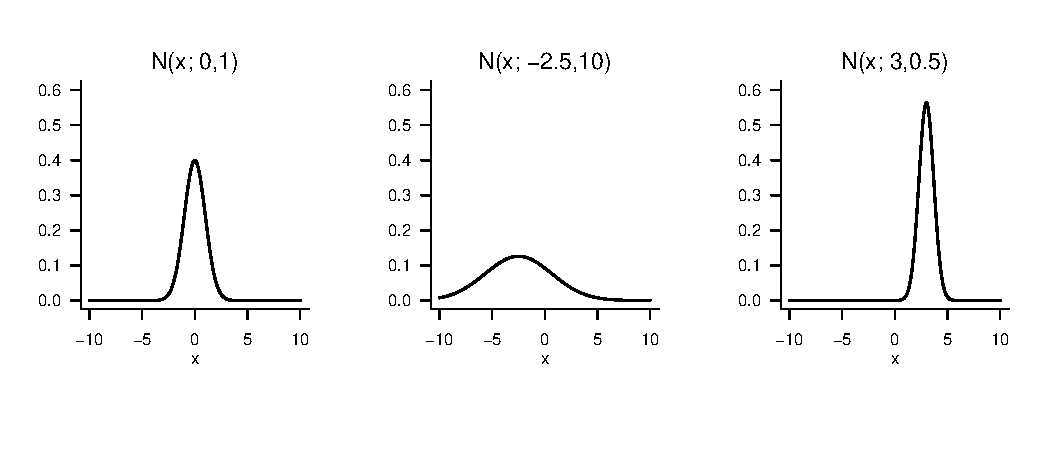
\includegraphics[width=1\linewidth]{4_Abbildungen/wtfi_4_normalverteilung_wdf} \end{center}
\end{frame}

\begin{frame}{Wahrscheinlichkeitsdichtefunktionen}
\protect\hypertarget{wahrscheinlichkeitsdichtefunktionen-3}{}
\small
\begin{definition}[Gamma-Zufallsvariable]
\justifying
Es sei $\xi$ eine Zufallsvariable mit Ergebnisraum $\mathcal{X} := \mathbb{R}_{>0}$ und WDF
\begin{equation}
p : \mathbb{R}_{>0} \to \mathbb{R}_{>0},  x \mapsto p(x) :=
\frac{1}{\Gamma(\alpha)\beta^{\alpha}}x^{\alpha-1}\exp\left(-\frac{x}{\beta}\right),
\end{equation}
wobei $\Gamma$ die Gammafunktion bezeichne. Dann sagen wir, dass $\xi$ einer
\textit{Gammaverteilung mit Formparameter $\alpha >0$ und Skalenparameter $\beta > 0$}
unterliegt und nennen $\xi$ eine \textit{gammaverteilte Zufallsvariable}. Wir kürzen
dies mit $\xi \sim G(\alpha,\beta)$ ab. Die WDF einer gammaverteilen Zufallsvariable
bezeichnen wir mit
\begin{equation}
G(x;\alpha,\beta) := \frac{1}{\Gamma(\alpha)\beta^{\alpha}}x^{\alpha-1}\exp\left(-\frac{x}{\beta}\right).
\end{equation}
\end{definition}

Bemerkung

\begin{itemize}
\item $G\left(\frac{n}{2},2\right)$ heißt auch \textit{Chi-Quadrat ($\chi^2$) Verteilung mit $n$ Freiheitsgraden}.
\end{itemize}
\end{frame}

\begin{frame}{Wahrscheinlichkeitsdichtefunktionen}
\protect\hypertarget{wahrscheinlichkeitsdichtefunktionen-4}{}
Gamma-Zufallsvariablen \vspace{1cm}

\begin{center}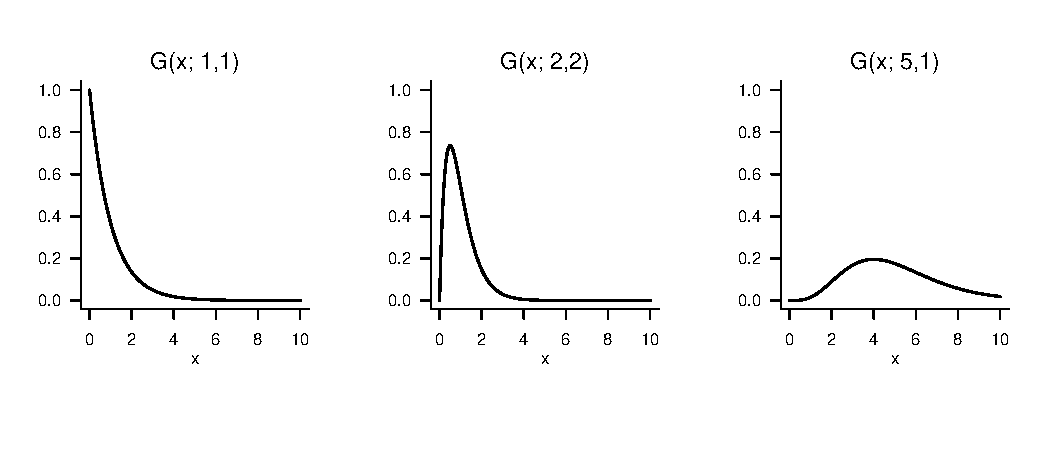
\includegraphics[width=1\linewidth]{4_Abbildungen/wtfi_4_gammaverteilung_wdf} \end{center}
\end{frame}

\begin{frame}{Wahrscheinlichkeitsdichtefunktionen}
\protect\hypertarget{wahrscheinlichkeitsdichtefunktionen-5}{}
\small
\begin{definition}[Beta-Zufallsvariable]
\justifying
Es sei $\xi$ eine Zufallsvariable mit Ergebnisraum $\mathcal{X} := [0,1]$ und WDF
\begin{equation}
p : \mathcal{X} \to [0,1], x \mapsto p(x)
:= \frac{\Gamma(\alpha + \beta)}{\Gamma(\alpha)\Gamma(\beta)}
x^{\alpha-1}(1-x)^{\beta-1} \mbox{ mit } \alpha,\beta \in \mathbb{R}_{>0},
\end{equation}
wobei $\Gamma$ die Gammafunktion bezeichne. Dann sagen wir, dass $\xi$ einer
\textit{Beta-Verteilung} mit Parametern $\alpha >0$ und $\beta>0$ unterliegt,
und nennen $\xi$ eine beta-verteilte Zufallsvariable. Wir kürzen dies mit
$\xi \sim \mbox{Beta}(\alpha,\beta)$ ab. Die WDF einer beta-verteilten Zufallsvariable
bezeichnen wir mit
\begin{equation}
\mbox{Beta}(x;\alpha,\beta)
:= \frac{\Gamma(\alpha + \beta)}{\Gamma(\alpha)\Gamma(\beta)}
x^{\alpha-1}(1-x)^{\beta-1}.
\end{equation}
\end{definition}

Bemerkung

\begin{itemize}
\item Für $\alpha < 1, \beta < 1$ ist der Ergebnisraum $\mathcal{X} := ]0,1[$.
\end{itemize}
\end{frame}

\begin{frame}{Wahrscheinlichkeitsdichtefunktionen}
\protect\hypertarget{wahrscheinlichkeitsdichtefunktionen-6}{}
Beta-Zufallsvariable \vspace{1cm}

\begin{center}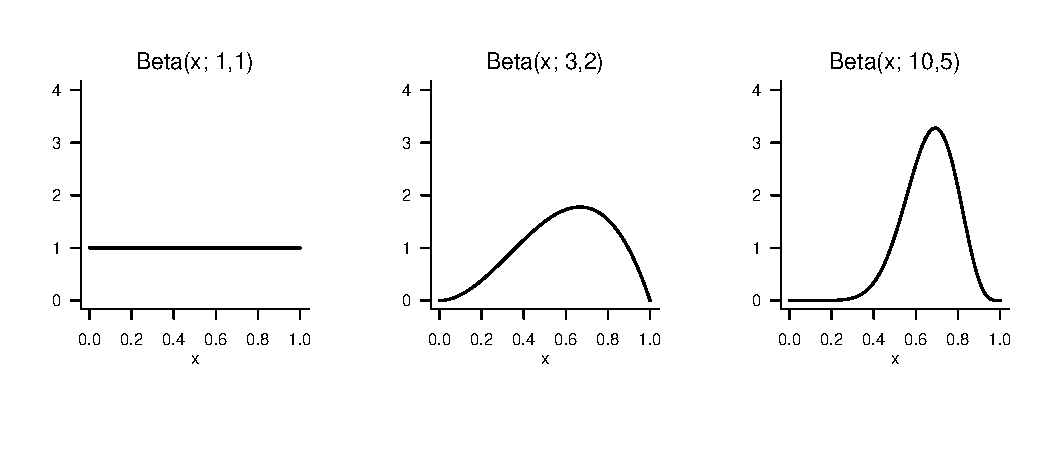
\includegraphics[width=1\linewidth]{4_Abbildungen/wtfi_4_betaverteilung_wdf} \end{center}
\end{frame}

\begin{frame}{Wahrscheinlichkeitsdichtefunktionen}
\protect\hypertarget{wahrscheinlichkeitsdichtefunktionen-7}{}
\small
\begin{definition}[Gleichverteilte Zufallsvariable]
\justifying
Es sei $\xi$ eine kontinuierliche Zufallsvariable mit Ergebnisraum $\mathbb{R}$ und WDF
\begin{equation}
p : \mathbb{R} \to \mathbb{R}_{\ge 0}, x\mapsto p(x) :=
\begin{cases}
\frac{1}{b - a} & x \in [a,b] \\
0               & x \notin [a,b]
\end{cases}.
\end{equation}

Dann sagen wir, dass $\xi$ einer \textit{Gleichverteilung mit Parametern $a$ und $b$}
unterliegt und nennen $\xi$ eine \textit{gleichverteilte Zufallsvariable}. Wir
kürzen dies mit $\xi \sim U(a,b)$ ab. Die WDF einer gleichverteilten Zufallsvariable
bezeichnen wir mit
\begin{equation}
U(x;a,b) := \frac{1}{b - a}.
\end{equation}
\end{definition}
\end{frame}

\begin{frame}{Wahrscheinlichkeitsdichtefunktionen}
\protect\hypertarget{wahrscheinlichkeitsdichtefunktionen-8}{}
Gleichverteilte Zufallsvariablen \vspace{1cm}

\begin{center}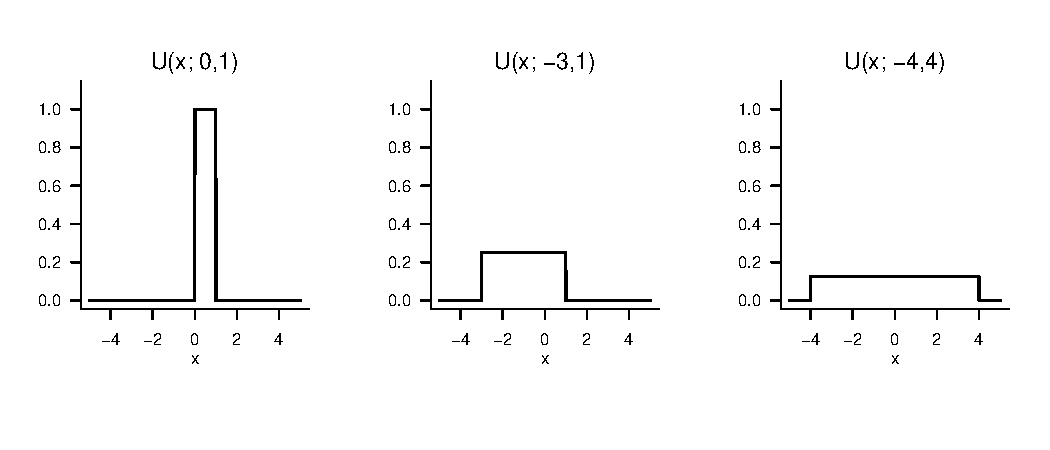
\includegraphics[width=1\linewidth]{4_Abbildungen/wtfi_4_gleichverteilung_wdf} \end{center}
\end{frame}

\begin{frame}{}
\protect\hypertarget{section-8}{}
\large
\setstretch{2.7}
\vfill

Konstruktion, Definition, Notation, Intuition

Wahrscheinlichkeitsmassefunktionen

Wahrscheinlichkeitsdichtefunktionen

\textbf{Kumulative Verteilungsfunktionen}

Selbstkontrollfragen \vfill
\end{frame}

\begin{frame}{Kumulative Verteilungsfunktionen}
\protect\hypertarget{kumulative-verteilungsfunktionen}{}
\small
\begin{definition}[Kumulative Verteilungsfunktion]
\justifying
Die \textit{kumulative Verteilungsfunktion (KVF)} einer Zufallsvariable $\xi$ ist definiert als
\begin{equation}
P : \mathbb{R} \to [0,1], x \mapsto P(x) := \mathbb{P}(\xi \le x).
\end{equation}
\end{definition}

Bemerkungen

\begin{itemize}
\item KVFen sind sowohl für diskrete als auch kontinuierliche ZVen definiert.
\item $P(x)$ ist für jedes $x \in \mathbb{R}$ definiert, auch wenn $x \notin \mathcal{X}$.
\item Mithilfe von KVFen können Intervallwahrscheinlichkeiten angegeben werden
\end{itemize}
\end{frame}

\begin{frame}{Kumulative Verteilungsfunktionen}
\protect\hypertarget{kumulative-verteilungsfunktionen-1}{}
\small
\begin{theorem}[Überschreitungswahrscheinlichkeit]
\justifying
\normalfont
Es sei $\xi$ eine Zufallsvariable mit Ereignisraum $\mathcal{X}$ und $P$
ihre kumulative Verteilungsfunktion. Dann gilt für die \textit{Überschreitungswahrscheinlichkeit}
$\mathbb{P}(\xi > x)$, dass
\begin{equation}
\mathbb{P}(\xi > x) = 1 - P(x) \mbox{ für alle } x \in \mathcal{X}.
\end{equation}
\end{theorem}

\footnotesize

\underline{Beweis} \vspace{1mm}

Die Ereignisse \(\{\xi > x\}\) und \(\{\xi \le x\}\) sind disjunkt und
\begin{equation}
\Omega
= \{\omega\in \Omega| \xi(\omega) > x\} \cup \{\omega\in \Omega|\xi(\omega) \le x\}
= \{\xi > x\} \cup \{\xi \le x\}.
\end{equation}

Mit der \(\sigma\)-Additivität von \(\mathbb{P}\) folgt dann
\begin{align}
\begin{split}
\mathbb{P}(\Omega) & = 1                                \\
\Leftrightarrow
\mathbb{P}( \{\xi > x\} \cup \{\xi \le x\}) & = 1           \\
\Leftrightarrow
\mathbb{P}(\{\xi > x\}) + \mathbb{P}(\{\xi \le x\}) & = 1   \\
\Leftrightarrow
\mathbb{P}(\{\xi > x\}) &  =  1 -  \mathbb{P}(\{\xi \le x\}) \\
\Leftrightarrow
\mathbb{P}(\{\xi > x\}) &  =  1 -  P(x).
\end{split}
\end{align} \(\hfill \Box\)
\end{frame}

\begin{frame}{Kumulative Verteilungsfunktionen}
\protect\hypertarget{kumulative-verteilungsfunktionen-2}{}
\small
\begin{theorem}[Intervallwahrscheinlichkeiten]
\justifying
\normalfont
Es sei $\xi$ eine Zufallsvariable mit Ereignisraum $\mathcal{X}$ und $P$ ihre
kumulative Verteilungsfunktion. Dann gilt für die \textit{Intervallwahrscheinlichkeit}
$\mathbb{P}(\xi \in \,]x_1,x_2])$, dass
\begin{equation}
\mathbb{P}(\xi \in \, ]x_1,x_2]) = P(x_2) - P(x_1)
\mbox{ für alle } x_1,x_2 \in \mathcal{X}
\mbox{ mit } x_1 < x_2.
\end{equation}
\end{theorem}

\footnotesize

\underline{Beweis} \vspace{1mm}

Wir betrachten die Ereignisse
\(\{\xi \le x_1\}\),\(\{x_1 < \xi \le x_2\}\) und \(\{\xi \le x_2\}\),
wobei \begin{equation}
\{\xi \le x_1\} \cap \{x_1 < \xi \le x_2\} = \emptyset
\mbox{ und }
\{\xi \le x_1\} \cup \{x_1 < \xi \le x_2\} = \{\xi \le x_2\}.
\end{equation} gelten. Mit der \(\sigma\)-Additivität von \(\mathbb{P}\)
gilt dann \begin{align}
\begin{split}
\mathbb{P}(\{\xi \le x_1\} \cup \{x_1 < \xi \le x_2\}) & = \mathbb{P}(\{\xi \le x_2\})              \\
\Leftrightarrow
\mathbb{P}(\{\xi \le x_1\}) + \mathbb{P}(\{x_1 < \xi \le x_2\}) & = \mathbb{P}(\{\xi \le x_2\})         \\
\Leftrightarrow
\mathbb{P}(\{x_1 < \xi \le x_2\}) & = \mathbb{P}(\{\xi \le x_2\}) - \mathbb{P}(\{\xi \le x_1\})         \\
\Leftrightarrow
\mathbb{P}(\{x_1 < \xi \le x_2\}) & = P(x_2) - P(x_1)                                           \\
\Leftrightarrow
\mathbb{P}(\xi \in \,]x_1,x_2]) & = P(x_2) - P(x_1).
\end{split}
\end{align} \(\hfill \Box\)
\end{frame}

\begin{frame}{Kumulative Verteilungsfunktionen}
\protect\hypertarget{kumulative-verteilungsfunktionen-3}{}
\small
\begin{theorem}[Eigenschaften von kumulative Verteilungsfunktionen]
\normalfont
Es sei $\xi$ eine Zufallsvariable und $P$ ihre kumulative Verteilungsfunktion.
Dann hat $P$ die folgenden Eigenschaften
\begin{itemize}
\item[(1)] $P$ ist \textit{monoton steigend}, i.e., wenn $x_1 < x_2$, dann gilt $P(x_1)\le P(x_2)$.
\item[(2)] $\lim_{x \to -\infty}P(x) = 0$ und $\lim_{x \to \infty}P(x) = 1$.
\item[(3)] $P$ ist \textit{rechtsseitig stetig}, d.h., $P(x) = P(x^+) = \lim_{y \to x, y > x} P(y)$ für alle $x \in \mathbb{R}$
\end{itemize}
\end{theorem}

Bemerkungen

\begin{itemize}
\item Die genannten Eigenschaften können auch zur Definition einer KVF genutzt werden.
\item (3) $\Leftrightarrow$
Eine KVF hat keine Sprünge, wenn man sich Grenzpunkten von rechts nähert.
\end{itemize}
\end{frame}

\begin{frame}{Kumulative Verteilungsfunktionen}
\protect\hypertarget{kumulative-verteilungsfunktionen-4}{}
\footnotesize

\underline{Beweis} \vspace{2mm}

\begin{enumerate}
[(1)]
\item
  Wir halten zunächst fest, dass für Ereignisse \(A \subset B\) gilt,
  dass \(\mathbb{P}(A)\le \mathbb{P}(B)\). Wie halten dann fest, dass
  für \(x_1 < x_2\), \begin{equation}
  \{\xi \le x_1\} =
  \{\omega \in \Omega|\xi(\omega)\le x_1\} \subset
  \{\omega \in \Omega|\xi(\omega)\le x_2\} =
  \{\xi \le x_2\}
  \end{equation} Also gilt \begin{equation}
  \mathbb{P}(\{\xi \le x_1\})
  \le
  \mathbb{P}\{\xi \le x_2\}
  \Rightarrow P(x_1) \le P(x_2).
  \end{equation}
\item
  Wir verzichten auf einen Beweis \vspace{2mm}
\item
  Wir definieren \begin{equation}
  P(x^+) = \lim_{y \to x, y > x} P(y).
  \end{equation} Seien nun \(y_1 > y_2 > \cdots\) so, dass
  \(\lim_{n \to \infty}y_n = x\). Dann gilt \begin{equation}
  \{\xi \le x\} = \cap_{n = 1}^\infty \{\xi \le y_n\}.
  \end{equation} Es gilt also \begin{equation}
  P(x)
  = \mathbb{P}(\{\xi \le x\})
  = \mathbb{P}(\cap_{n = 1}^\infty \{\xi \le y_n\})
  = \lim_{n\to \infty}\mathbb{P}(\{\xi \le y_n\})
  = P(x^+),
  \end{equation} wobei wir die dritte Gleichung unbegründet stehen
  lassen.
\end{enumerate}
\end{frame}

\begin{frame}{Kumulative Verteilungsfunktionen}
\protect\hypertarget{kumulative-verteilungsfunktionen-5}{}
Kumulative Verteilungsfunktionen von diskreten Zufallsvariablen
\setstretch{2.7} \small

\begin{itemize}
\item Wenn $a < b$ und $\mathbb{P}(a < \xi < b) = 0$, dann ist $P$ konstant horizontal auf $]a,b[$.
\item An jedem Punkt $x$ mit $\mathbb{P}(\xi=x)>0$ springt die KVF um den Betrag $\mathbb{P}(\xi=x)$.
\item $\Leftrightarrow$ An jedem Punkt $x$ mit $p(x)>0$ springt die KVF um den Betrag $p(x)>0$.
\item Generell ist die KVF einer diskreten Zufallsvariable mit Ergebnisraum $\mathbb{N}_0$ durch
\begin{equation}
P : \mathbb{R} \to [0,1], x \mapsto P(x) := \sum_{k=0}^{\lfloor x  \rfloor} \mathbb{P}(\xi = k)
\end{equation}
gegeben, wobei $\lfloor x \rfloor$ die Abrundungsfunktion bezeichnet.
\end{itemize}
\end{frame}

\begin{frame}{Kumulative Verteilungsfunktionen}
\protect\hypertarget{kumulative-verteilungsfunktionen-6}{}
Bernoulli-Zufallsvariablen \vspace{.2cm}

\begin{center}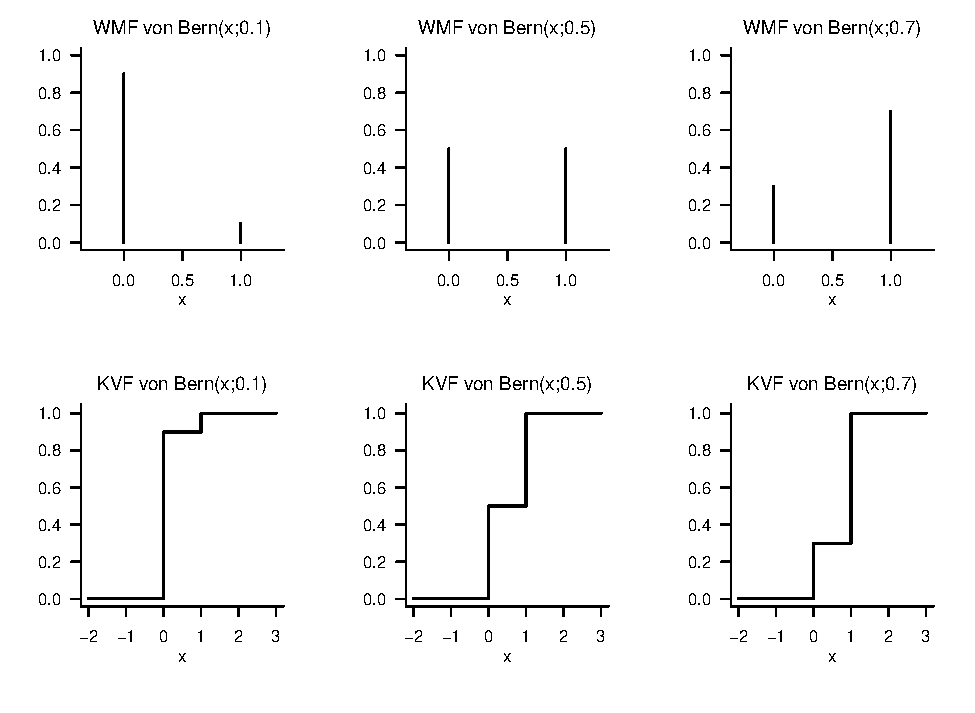
\includegraphics[width=0.8\linewidth]{4_Abbildungen/wtfi_4_bernoulliverteilung_kvf} \end{center}
\end{frame}

\begin{frame}{Kumulative Verteilungsfunktionen}
\protect\hypertarget{kumulative-verteilungsfunktionen-7}{}
Binomial-Zufallsvariablen \vspace{.2cm}

\begin{center}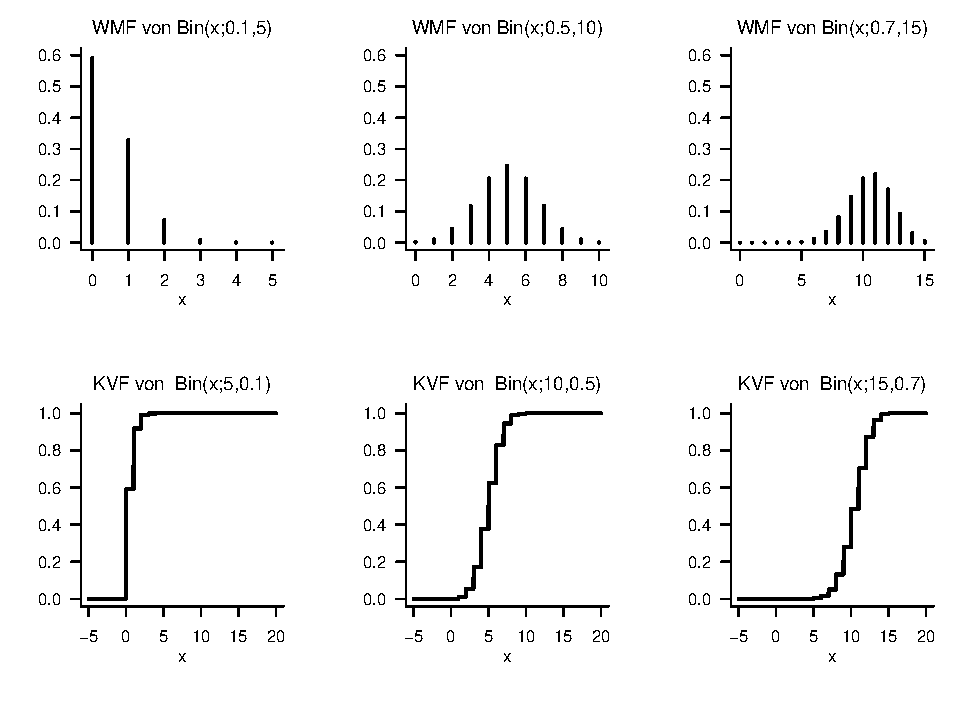
\includegraphics[width=0.8\linewidth]{4_Abbildungen/wtfi_4_binomialverteilung_kvf} \end{center}
\end{frame}

\begin{frame}{Kumulative Verteilungsfunktionen}
\protect\hypertarget{kumulative-verteilungsfunktionen-8}{}
\small
\begin{theorem}[Kumulative Verteilungsfunktionen von kontinuierlichen ZVen]
\justifying
\normalfont
$\xi$ sei eine kontinuierliche Zufallsvariable mit WDF $p$ und KVF $P$. Dann gilt
\begin{equation}
P(x) = \int_{-\infty}^x p(t)\,dt
\mbox{ und }
p(x) = \frac{d}{dx}P(x).
\end{equation}
\end{theorem}

\footnotesize

\underline{Beweis} \vspace{1mm}

Wir halten zunächst fest, dass weil \(\mathbb{P}(\xi = x) = 0\) für alle
\(x \in \mathbb{R}\) gilt, die KVF von \(\xi\) keine Sprünge hat, d.h.
\(P\) ist stetig. Mit der Definitionen von WDF und KVF, folgt, dass
\(P\) die Form einer Stammfunktion von \(p\) hat. Dass \(p\) die
Ableitung von \(P\) ist, folgt dann unmittelbar aus dem Fundamentalsatz
der Analysis.

\(\hfill \Box\)

Bemerkungen

\begin{itemize}
\item Die KVF ist eine Stammfunktion der WDF, die WDF ist die Ableitung der KVF.
\item Das \textit{Theorem von Radon-Nikodym} ist eine generalisierte Variante dieser Einsicht.
\item KVFen von kontinuierlichen ZV heißen auch kumulative Dichtefunktionen (KDFen).
\end{itemize}
\end{frame}

\begin{frame}{Kumulative Verteilungsfunktionen}
\protect\hypertarget{kumulative-verteilungsfunktionen-9}{}
\begin{large}
Beispiel (Normalverteilung)
\end{large}

\small
\justifying

Es sei \(X \sim N(\mu,\sigma^2)\). \setstretch{1.6}

\begin{itemize}
\item Die WDF von $\xi$ ist
\begin{equation*}
p : \mathbb{R} \to \mathbb{R}_{>0}, x \mapsto p(x)
:= \frac{1}{\sqrt{2\pi\sigma^2}}\exp\left(-\frac{1}{2\sigma^2}(x-\mu)^2\right).
\end{equation*}
\item Die KVF von $\xi$ ist
\begin{align*}
\begin{split}
P : \mathbb{R} \to ]0,1[, x \mapsto P(x)
 = \frac{1}{\sqrt{2\pi\sigma^2}}\int_{-\infty}^x\exp\left(-\frac{1}{2\sigma^2}(\xi-\mu)^2\right) \,d\xi
\end{split}.
\end{align*}
\item Die KVF von $\xi \sim N(\mu,\sigma^2)$ kann nur numerisch, nicht analytisch, berechnet werden.
\item Für $\mu = 1, \sigma^2 = 1$, gilt zum Beispiel $p(2) = 0.24$ und $P(2) = 0.84$.
\item Die WDF und KVF von $Z \sim N(0,1)$ werden oft mit  $\phi$ und $\Phi$, respektive, bezeichnet.
\end{itemize}
\end{frame}

\begin{frame}{Kumulative Verteilungsfunktionen}
\protect\hypertarget{kumulative-verteilungsfunktionen-10}{}
Normalverteilte Zufallsvariablen \vspace{.2cm}

\begin{center}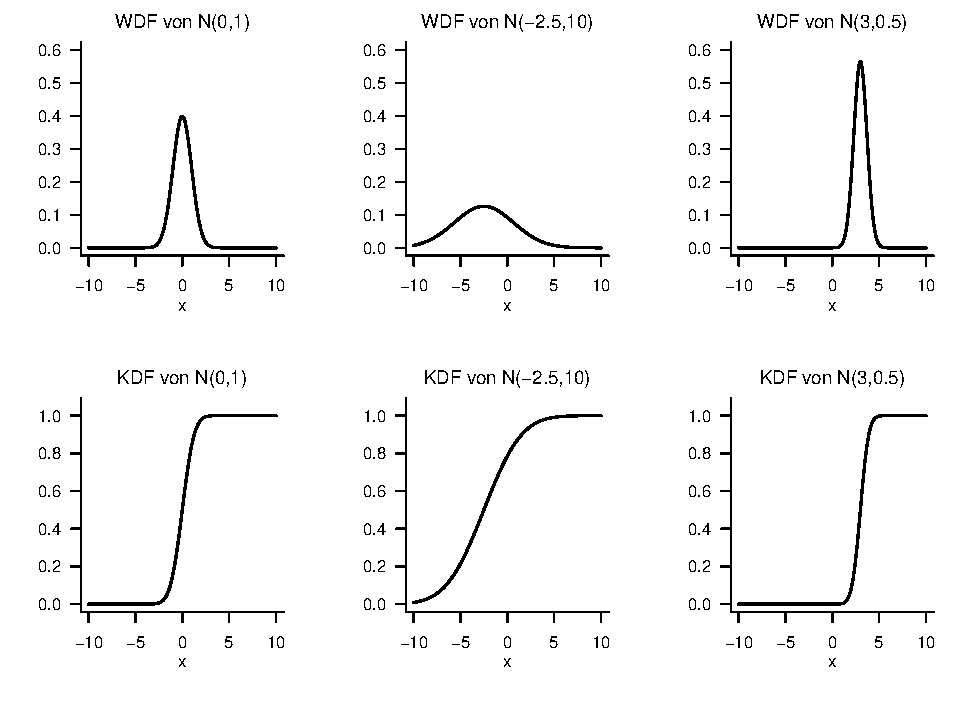
\includegraphics[width=0.8\linewidth]{4_Abbildungen/wtfi_4_normalverteilung_kvf} \end{center}
\end{frame}

\begin{frame}{Kumulative Verteilungsfunktionen}
\protect\hypertarget{kumulative-verteilungsfunktionen-11}{}
\small
\begin{definition}[Inverse Kumulative Verteilungsfunktion]
$\xi$ sei eine kontinuierliche Zufallsvariable mit KVF $P$. Dann heißt die Funktion
\begin{equation}
P^{-1} : ]0,1[ \to \mathbb{R}, q \mapsto P^{-1}(q) := \{x \in \mathbb{R}|P(x) = q\}
\end{equation}
die \textit{inverse kumulative Verteilungsfunktion von $\xi$}.
\end{definition}
\vspace{.1cm}

Bemerkungen

\begin{itemize}
\item $P^{-1}$ ist die Inverse von $P$, d.h. $P^{-1}(P(x)) = x$.
\item Offenbar gilt $P(x) = q \Leftrightarrow \mathbb{P}(\xi \le x) = q$.
\item Für $q \in ]0,1[$ ist also $P^{-1}(q)$ der Wert $x$ von $\xi$, so dass $\mathbb{P}(\xi \le x) = q$ gilt.
\item Wenn $Z \sim N(0,1)$ mit KVF $\Phi$ ist, dann gilt zum Beispiel $\Phi^{-1}(0.975) = 1.960$.
\end{itemize}
\end{frame}

\begin{frame}{Kumulative Verteilungsfunktionen}
\protect\hypertarget{kumulative-verteilungsfunktionen-12}{}
Beispiel (Normalverteilung) \vspace{2mm}

\small
\justifying

Es sei \(\xi \sim N(\mu,\sigma^2)\).

\begin{itemize}
\item Die KVF von $\xi$ ist
\begin{equation}
P : \mathbb{R} \to ]0,1[, x \mapsto \mathbb{P}(\xi \le x)
= \frac{1}{\sqrt{2\pi\sigma^2}}\int_{-\infty}^x\exp\left(-\frac{1}{2\sigma^2}(\xi-\mu)^2\right) \,d\xi
\end{equation}

\item Die inverse KVF von $\xi$ ist
\begin{equation}
P^{-1} : ]0,1[ \to \mathbb{R}, q \mapsto P^{-1}(q) = \{x \in \mathbb{R}|P(x) = q\}.
\end{equation}

\item Für $\mu = 1, \sigma^2 = 1$ gilt z.B., dass $P(2) = 0.84$ und $P^{-1}(0.84) = 2$.

\item Die inverse KVF von $\xi \sim N(0,1)$ wird oft mit $\Phi^{-1}$ bezeichnet.

\item Typische Beispielwerte für die KVF und inverse KVF  von $N(0,1)$ sind
\begin{itemize}
\footnotesize
\item $\Phi(1.645) = 0.950$, $\Phi^{-1}(0.950) = \Phi^{-1}(1 -0.050) = 1.645$.
\item $\Phi(1.960) = 0.975$, $\Phi^{-1}(0.975) = \Phi^{-1}(1 - \frac{0.050}{2})$.

\end{itemize}
\end{itemize}
\end{frame}

\begin{frame}{Kumulative Verteilungsfunktionen}
\protect\hypertarget{kumulative-verteilungsfunktionen-13}{}
Normalverteilte Zufallsvariablen \vspace{.2cm}

\begin{center}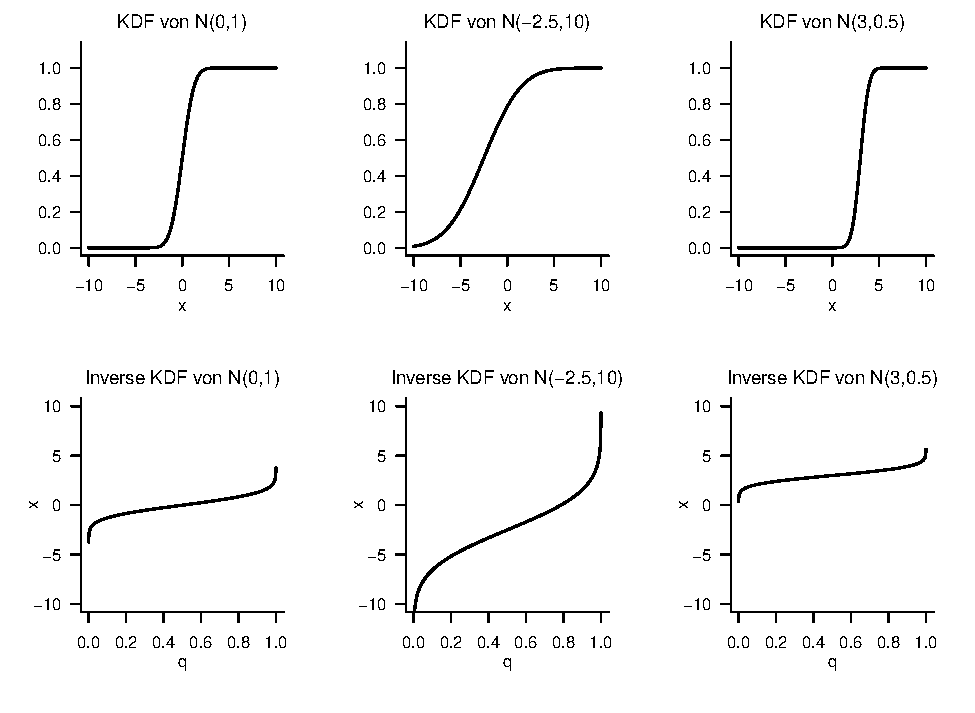
\includegraphics[width=0.8\linewidth]{4_Abbildungen/wtfi_4_normalverteilung_ikvf} \end{center}
\end{frame}

\begin{frame}{}
\protect\hypertarget{section-9}{}
\large
\setstretch{2.7}
\vfill

Konstruktion, Definition, Notation, Intuition

Wahrscheinlichkeitsmassefunktionen

Wahrscheinlichkeitsdichtefunktionen

Kumulative Verteilungsfunktionen

\textbf{Selbstkontrollfragen}
\end{frame}

\begin{frame}{Selbstkontrollfragen}
\protect\hypertarget{selbstkontrollfragen}{}
\small
\setstretch{1.7}
\begin{enumerate}
\item Definieren Sie den Begriff der Zufallsvariable.
\item Erläutern Sie die Gleichung $\mathbb{P}_\xi(\xi = x) = \mathbb{P}(\{\xi = x\})$.
\item Erläutern Sie die Bedeutung von $\mathbb{P}(\xi = x)$.
\item Definieren Sie den Begriff der Wahrscheinlichkeitsmassefunktion.
\item Definieren Sie die Begriffe der Wahrscheinlichkeitsdichtefunktion.
\item Definieren Sie den Begriff der kumulativen Verteilungsfunktion.
\item Schreiben sie die Intervallwahrscheinlichkeit einer Zufallsvariable mithilfer ihrer KVF. 
\item Definieren Sie die WDF und KVF einer normalverteilten Zufallsvariable.
\item Schreiben Sie den Wert $P(x)$ der KVF einer Zufallsvariable mithilfe ihrer WDF.
\item Schreiben Sie den Wert $p(x)$ der WDF einer Zufallsvariable mithilfe ihrer KVF.
\item Definieren Sie den Begriff der inversen Verteilungsfunktion.
\end{enumerate}
\end{frame}

\begin{frame}{Referenzen}
\protect\hypertarget{referenzen}{}
\footnotesize

\hypertarget{refs}{}
\begin{CSLReferences}{1}{0}
\leavevmode\vadjust pre{\hypertarget{ref-hesse_2009}{}}%
Hesse, Christian. 2009. \emph{Wahrscheinlichkeitstheorie}. 2nd ed.
Wiesbaden: Vieweg + Teubner.

\end{CSLReferences}
\end{frame}

\end{document}
